%% ============================================================================
%% RESS revision — complete revised manuscript (LaTeX build of the proposed edits)
%% Built 2026-07-28 from RESS_Paper__New_.docx + RESS_edit_proposals.md (EDITs 1-18).
%% The original docx is untouched; this file is the applied revision.
%%
%% HIGHLIGHTS (for the journal's separate highlights file):
%%  - Exact source-to-node reliability for DAGs with reconvergent dependencies,
%%    verified to floating-point precision against an independent exact
%%    decision-diagram method
%%  - Formally positioned as a specialisation of cutset conditioning, with
%%    per-instance cost determined by the conditioning-set width -- the same
%%    parameter that governs well-ordered decision diagrams
%%  - Native propagation of imprecise component reliabilities: exact interval
%%    ranges and guaranteed probability-box bounds
%%  - Certified bounds on decision-relevant reliability probabilities from a
%%    single propagation, without simulation
%%  - Applied case study of a medical drone logistics network for Scotland,
%%    locating the practical redundancy boundary of exact analysis
%%
%% TODO(author): affiliations below are placeholders -- copy the exact
%% affiliation/footnote block from the submission system version. STILL OPEN
%% as of the 2026-09-06 pre-write audit -- not resolvable without the original
%% submission record (see pre-write final/README.md item 5).
%% RESOLVED 2026-09-06: dPrPm bound columns in tab:grid_accuracy filled in
%% directly from Tong & Tien (2019) Table 2 (source PDF, page 7) -- see
%% pre-write final/manuscript/CORRECTIONS_APPLIED.md item 2.
%% ============================================================================
\documentclass[preprint,12pt]{elsarticle}

\usepackage{amsmath,amssymb,amsthm}
\usepackage{booktabs}
\usepackage{graphicx}
\usepackage{caption}
\usepackage{subcaption}
\usepackage{algorithm}
\usepackage{algpseudocode}
\usepackage{tikz}
\usepackage{pgfplots}
\pgfplotsset{compat=1.18}
\graphicspath{{figures/}}

\newtheorem{lemma}{Lemma}
\theoremstyle{definition}
\newtheorem{definition}{Definition}
\newtheorem{assumption}{Assumption}

\journal{Reliability Engineering \& System Safety}

\begin{document}
\begin{frontmatter}

\title{Information Propagation Algorithm for Exact Reliability Analysis in Directed Acyclic Process Networks}

\author[strath]{Temitope Ohiani}
\author[strath]{Edoardo Patelli}
\author[strath]{Caroline Pyke}
\address[strath]{University of Strathclyde, Glasgow, United Kingdom}

\begin{abstract}
Reliability analysis in directed acyclic process networks requires computing, for each node, the
probability that at least one viable path exists from any source node to that node. Standard analytical
formulations become inaccurate or inefficient in the presence of reconvergent path structures, where
multiple paths diverge from shared upstream ancestors and reconverge downstream, creating statistical
dependencies that violate path-independence assumptions.
This paper presents the Information Propagation Algorithm (IPA), an exact message-passing method that
resolves these dependencies through conditional enumeration on shared fork ancestors. IPA processes the
network in topological order, identifying reconvergent (diamond) substructures, solving them by
conditioning on a minimal separating set, and replacing them with statistically equivalent supernodes.
The method is shown to be a specialisation of cutset conditioning to source-to-node reachability: its
per-instance cost is exactly determined by the conditioning-set sizes encountered, a width parameter that
also governs the size of a well-ordered binary decision diagram on the same network. Exactness is
verified against an independent reduced-ordered binary decision diagram across a corpus of 129 random
directed acyclic graphs, six topological families, and several real infrastructure networks, with worst
observed disagreement at floating-point precision. The distinguishing capability of the method is the
native propagation of imprecise component reliabilities: interval-valued inputs yield the exact
reliability range, a consequence of the monotonicity of the reachability function, and probability-box
inputs yield guaranteed distributional bounds through a conditioning operator built on the
Fr\'echet--Hoeffding inequalities, enabling certified bounds on decision-relevant probabilities that
point-valued exact methods cannot produce analytically.
The method is applied to a medical drone logistics network for Scotland in which every input is derived
from the source design study. Propagated reliability bounds identify the locations whose delivery
reachability is most uncertain, and a sweep of a network-redundancy design parameter locates the
practical boundary of exact computation on this real network; within the range tested, the proposed
method remains practical at a redundancy level at which the decision-diagram alternative did not complete
within a practical computational budget.
\end{abstract}

\begin{keyword}
Network Reliability \sep Directed Acyclic Graphs \sep Message Passing \sep Reconvergent Structures \sep
Imprecise Probability \sep Process Networks \sep Infrastructure Systems
\end{keyword}

\end{frontmatter}

%% ============================================================================
\section{Introduction}\label{sec:intro}

Many infrastructure and engineered systems operate through the propagation of resources, services, or
information across interconnected components. Examples include electric power networks, water
distribution systems, telecommunication networks, transportation systems, and logistics networks. In such
systems, functionality depends not only on the reliability of individual components but also on the
existence of viable directed paths through which flow can propagate from source nodes to downstream
nodes. In this paper, we refer to this class of systems as multi-source process networks. Failures in
these systems can have severe operational, economic, environmental, and societal consequences. Their
assessment therefore requires metrics that quantify not only component reliability but also the ability
of the network to preserve connectivity and sustain flow. A natural reliability measure in this context
is the probability that at least one viable path exists from one or more source nodes to a given target
node. This source-to-node reachability reliability provides a direct measure of the network's ability to
maintain function under component and transmission failures.

Directed acyclic graphs (DAGs) are a natural fit to model and evaluate the performance of resource flow
systems. In a DAG, nodes represent system components, processing stages, or transfer locations, while
directed edges model permissible flow transitions and dependencies between components. Consider the
typical process of transport networks where service at downstream locations may depend on the successful
operation of several upstream links, hubs, or transfer stages. Failures at earlier stations can cause
disruption and delays in travel and, in some cases, stop service altogether.

To mitigate cascading failure scenarios and service bottlenecks, the reliability of the network's
resource flow is an important performance metric to monitor. Reliability is generally defined as the
probability that a system performs its intended function over a specified time. In flow networks, the
intended function is that the other parts of the network successfully receive information flowing from
the sources. Complex systems have redundancy strategies and backup paths to ensure this flow. Reliability
in multi-source flow networks is related to the probability that at least one viable operational path
exists from source nodes to the other nodes in the network.

The classic approach to exactly solving the reliability problem involves enumerating and combining all
possible source-to-node paths. However, this quickly becomes computationally intractable for complex
process systems with multiple sources, extensive redundancy, and re-convergent network topologies
(George-Williams et al.\ 2021). In particular, when distinct paths share upstream nodes or edges before
reconverging downstream, the resulting path events are no longer independent, and na\"ive
path-combination rules become invalid.

The structure of DAGs suggests an alternative viewpoint based on message passing. Rather than globally
enumerating all viable paths, reliability can be computed locally and recursively by asking, at each
node: what is the probability that at least one viable signal reaches this node from any source? For
tree-like or conditionally independent substructures, this can be evaluated efficiently using local
update rules. However, reconvergent path structures remain problematic because they induce statistical
dependencies between incoming signals. These dependencies must be resolved exactly if message passing is
to remain accurate.

This paper presents the Information Propagation Algorithm (IPA), an exact message-passing method for
reliability analysis in directed acyclic process networks. IPA exploits topological ordering to propagate
source-to-node reliability from upstream to downstream nodes. Its central idea is to identify
reconvergent fork--join subgraphs, referred to here as diamond structures, and resolve their dependency
explicitly by conditioning on the shared fork ancestors. Once solved, these diamond subgraphs are
replaced with statistically equivalent supernodes, allowing the network to be progressively simplified
without loss of exactness.

The proposed approach presents several advantages. First, it preserves exact reliability computation in
DAGs with reconvergent structures, avoiding the independence errors that arise from standard local update
rules. Second, by decomposing and caching repeated dependency patterns, it avoids repeated conditional
enumeration over already-resolved substructures, and its computational cost on a given network is
determined exactly, before enumeration begins, by the sizes of the conditioning sets its decomposition
identifies. Third, and distinctively, the propagation scheme extends beyond point-valued component
reliabilities: interval-valued reliabilities are propagated exactly, and probability-box (p-box)
reliabilities are propagated with guaranteed bounds, so that epistemic uncertainty about component data
can be carried through the analysis rather than suppressed into point estimates. These properties make
the method suitable for design-stage studies in which many network configurations must be assessed, and
for decision problems in which the reliability inputs themselves are only partially known.

\subsection{Related Works}\label{sec:related}

Early reliability analysis methods are based on relatively simple structural representations of systems.
The Reliability Block Diagram (RBD) (Billinton and Allan 1992; Rausand 2014; Ebeling 2019) method models
a system as interconnected component blocks arranged in series, parallel, or $k$-out-of-$n$
configurations, whose reliability can be computed using closed-form expressions. While computationally
efficient and intuitive, RBDs are limited in their ability to represent complex dependency structures and
reconvergent flows. Extensions such as Dynamic Reliability Block Diagrams (DRBD) (Distefano and Puliafito
2007) incorporate time-dependent behaviour, allowing for more realistic modelling of component
interactions and system dependencies, but they still struggle to represent highly interconnected networks
with multiple convergent paths.

Boolean logic-based methods provide a more flexible framework for modelling system failure mechanisms by
including event causes and consequences. Fault Tree Analysis (FTA) (Xing and Amari 2008) is a top-down
deductive logic tree to identify possible combinations of component failures that could cause specific
undesirable events. Event Tree Analysis (ETA) is the complementary inductive method where the logic tree
instead begins with the initiating event and systematically traces all possible sequences of subsequent
successes and failures through branching structures and logic gates (\v{C}epin 2011). These methods can
capture a wider range of logical dependencies than RBDs; however, for large-scale systems they require
extensive manual construction and become difficult to maintain. In addition, their computational cost
grows rapidly with the size and complexity of the logical expressions, particularly in systems with
multiple interacting pathways (Sherwin and Bossche 1993; Xing and Amari 2008).

The main limitations of tree-based methods stem from exponential growth in logic expressions and manual
construction requirements for complex systems. Binary Decision Diagrams (BDDs) (Rauzy 1993; Bryant 1986;
Brace et al.\ 1990) were adapted from circuit design to improve fault tree models by using variable
elimination and path reduction techniques on Boolean functions. In BDDs, Boolean functions are
represented as directed acyclic graphs based on Shannon decomposition, where each non-sink node
represents a Boolean variable with two outgoing edges corresponding to the variable being true or false
(Xing and Amari 2008). This structure allows BDD-based methods to require less memory and computational
time than traditional fault tree analysis (Rauzy 1993). BDD algorithms can handle complex Boolean
expressions with thousands of variables while maintaining polynomial space complexity for many systems.
However, their performance depends critically on variable ordering, and determining an optimal ordering
is itself computationally intractable in general (Bryant and Meinel 2002). For highly interconnected
networks with shared components and reconvergent fanout structures, BDD construction with diamond
structures --- where multiple independent paths converge at common nodes --- suffers from the
reconvergence problem, requiring extensive intermediate node generation that can exceed memory
limitations even for moderately sized systems. These computational challenges become particularly severe
when modelling common cause failures and complex dependency structures that propagate through multiple
interconnected pathways simultaneously.

Common cause failures create statistical dependencies that violate the independence assumptions
underlying traditional reliability calculations (Mosleh 1993). When multiple components share common
failure modes, the resulting dependency patterns cannot be efficiently captured through simple Boolean
combinations, representing a fundamental limitation shared by RBDs, FTAs, and BDDs in process systems
with convergent network topologies.

To overcome these limitations, path-based and graph-theoretic methods have been developed. These methods
contextualise the network as a probabilistic graph theory problem and leverage probability mathematics
and set operations to calculate network reliability. Exact methods based on minimal path sets and minimal
cut sets (Kumar et al.\ 2018; Li and Zhao 2005; Billinton and Allan 1992; Liu and Li 2012) identify the
smallest collections of components that ensure connectivity or guarantee system failure. Recursive
decomposition techniques further improve efficiency by partitioning the network into smaller subproblems.
For example, the cut-based method in Liu and Li (2012) proposes simultaneously using both the disjoint
minimal cut sets and disjoint minimal path sets during the decomposition process for networks with low
edge reliabilities. Kim and Kang's method (Kim and Kang 2013) extends the Recursive Decomposition
Algorithm through a Logical Expansion approach (LE-RDA) that uses two separate procedures for
intersection and union logical functions to handle decomposition of general system events with multiple
node pairs. Nevertheless, these methods remain computationally expensive for networks with extensive
redundancy and reconvergent connectivity, as they still require combinatorial enumeration of path or cut
structures.

Simulation methods such as Monte Carlo (MC) have become a widely adopted reliability analysis method for
complex networks (Fishman 1986). MC algorithms can handle arbitrary network structures and provide
confidence intervals, although they can become computationally expensive for large networks requiring
many samples to reach acceptable accuracy. Monte Carlo variants such as importance sampling (Hui 2007)
and subset simulation (Au and Beck 2001) have been proposed to address rare failure events, though these
optimisations often demand more computational cost.

More recently, message passing approaches based on probabilistic graphical models have been explored for
network reliability analysis (Yedidia et al.\ 2003; Pearl 1988). These methods infer the reliability of
the system by exploiting the network structure to propagate the local calculations throughout the network
until convergence. Unlike enumeration-based methods, message passing scales linearly with network size
and naturally handles complex dependency structures. For instance, methods for system reliability such as
the directed Probability Propagation Method (dPrPm) (Tong and Tien 2019) also allow dependencies to be
handled through pairwise probability tracking and approximation of joint distributions. While effective,
these approaches can become memory-intensive and computationally demanding as the number of dependent
interactions increases. In addition, convergence is not always guaranteed (Murphy et al.\ 2013), and
approximation quality depends heavily on network topology and component correlation strength.

In the exact-inference literature on probabilistic graphical models, dependencies induced by shared
ancestry are classically resolved either by conditioning --- cutset conditioning enumerates the states of
a set of variables whose removal renders the remaining structure singly connected (Pearl 1988) --- or by
clustering, as in the junction-tree algorithm, whose cost is exponential in the treewidth of the network
(Lauritzen and Spiegelhalter 1988). Both families are exact and both are governed by a structural width
parameter of the underlying graph. Section~\ref{sec:complexity} positions the present method within this
landscape: it is a specialisation of cutset conditioning to the source-to-node reachability problem, and
its realised cost is governed by the same width parameter that controls junction-tree inference and
well-ordered binary decision diagrams.

A further limitation cuts across all of the exact methods above: they operate on point-valued component
reliabilities. In practice, component failure probabilities are often known only imprecisely --- from
sparse data, expert elicitation, or manufacturer bounds --- and a rich literature on imprecise
probability represents such knowledge as intervals or as probability boxes (p-boxes), i.e.\ bounds on the
cumulative distribution of an uncertain quantity (Ferson et al.\ 2003). Arithmetic on p-boxes with known
or unknown dependence is formalised in Williamson and Downs (1990), building on the classical
Fr\'echet--Hoeffding bounds on joint distributions. Decision-diagram and path-based exact methods do not
propagate such imprecise inputs natively: an interval query requires repeated evaluation at selected
input corners, and no analytic route exists to a distributional bound. The method proposed here
propagates interval and p-box reliabilities directly, which is the capability that distinguishes it from
a well-ordered decision diagram of comparable computational cost.

Hence, existing methods face a trade-off between generality, computational efficiency, and exactness.
Classical analytical methods struggle with complex dependency structures, exact path-based approaches
suffer from combinatorial explosion, and simulation or approximate message-passing methods sacrifice
exactness for scalability. This work addresses this gap by proposing an exact message-passing framework
for DAG reliability analysis that explicitly resolves reconvergent dependencies through conditional
decomposition of fork--join substructures. By identifying and reducing these structures during
computation, the proposed method avoids repeated enumeration over shared dependencies while preserving
exact probabilistic results.

%% ============================================================================
\section{Network Model}\label{sec:model}

A process system is modelled as a directed acyclic graph $G=(V,E)$ where $V$ denotes the set of nodes
(components) and $E\subseteq V\times V$ represents the set of directed edges (dependencies). Let
$S\subseteq V$ denote the set of source and $T\subseteq V$ the sink nodes. Throughout the paper we use
$\mathrm{Pa}(v)$ and $\mathrm{Ch}(v)$ to represent the set of parent nodes and child nodes of $v$,
respectively.

\subsection{Component States and Probabilistic Model}

Each node $v\in V$ is associated with a binary random variable $X_v\in\{0,1\}$, where $X_v=1$ indicates
that node $v$ is operational. Similarly, each directed edge $(u,v)\in E$ is associated with a binary
random variable $X_{uv}\in\{0,1\}$ representing successful transmission from $u$ to $v$. We define:
\begin{itemize}
\item $R(v)=P(X_v=1)$: intrinsic reliability of node $v$;
\item $P(u,v)=P(X_{uv}=1)$: transmission probability of edge $(u,v)$.
\end{itemize}
A directed path $\pi(s,v)=(s=v_0,v_1,\dots,v_k=v)$ is said to be viable if all nodes and edges along the
path are operational, i.e.
\begin{equation}
X_{v_0}X_{v_1}\cdots X_{v_k}\cdot X_{v_0v_1}\cdots X_{v_{k-1}v_k}=1 .
\end{equation}

\begin{definition}[Viable Path]
A path $\pi(s,v)$ from source $s\in S$ to node $v\in V$ is viable if all nodes and edges along the path
are functional.
\end{definition}

\begin{figure}[t]
\centering
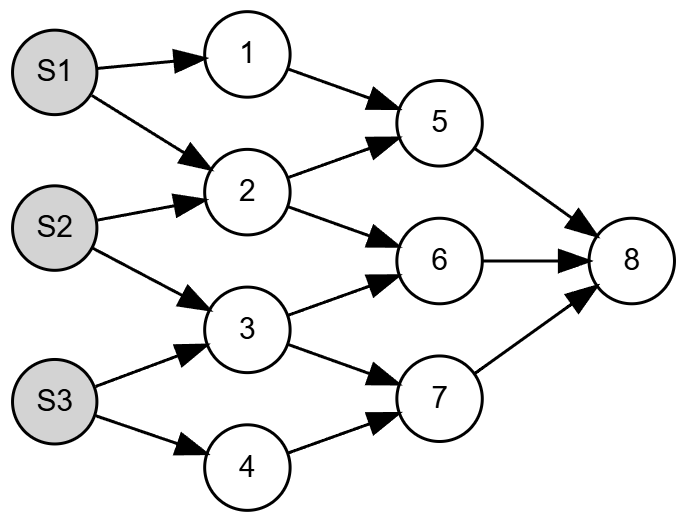
\includegraphics[width=0.6\linewidth]{rId11.png}
\caption{A multi-source directed acyclic graph.}
\label{fig:msdag}
\end{figure}

\subsection{Definition of Diamond Structures}

We formalise reconvergent dependency patterns through the notion of a diamond subgraph.

\begin{definition}[Diamond Structure]
A diamond structure is a subgraph $D\subseteq G$ characterised by:
a set of fork nodes $F\subseteq V$, where each $f\in F$ has at least two outgoing paths;
a join node $j\in V$ with at least two incoming paths;
at least two distinct directed paths from nodes in $F$ to $j$;
and at least one shared upstream node or edge among these paths.
\end{definition}

In such structures, the paths from fork nodes to the join node are not independent because they share
common components. The simplest case is a single-fork diamond, where all reconvergent paths originate
from a single fork node.

\subsection{Reliability Objective}\label{sec:objective}

The reliability problem is formally stated as computing the probability that there is at least one viable
path from any source node to each target node in the network. The reachability probability of a node
$v\in V$ is defined as the probability that at least one viable path exists from any source node to $v$:
\begin{equation}
b(v)=P\!\left(\bigcup_{s\in S}\ \bigcup_{\pi\in\Pi(s,v)}\{\pi \text{ is viable}\}\right),
\end{equation}
where $\Pi(s,v)$ denotes the set of all directed paths from $s$ to $v$. The quantity $b(v)$ represents
the probability that node $v$ successfully receives flow from at least one source and is referred to as
the node reliability (or belief) at $v$.

Equivalently, reachability can be expressed recursively. Define for each node the reachability indicator
\begin{equation}\label{eq:reach_indicator}
\mathcal{R}_v \;=\; X_v \wedge \Bigl( v\in S \ \vee\ \bigvee_{u\in \mathrm{Pa}(v)}
\bigl( \mathcal{R}_u \wedge X_{uv} \bigr) \Bigr),
\end{equation}
so that $b(v)=P(\mathcal{R}_v=1)$. Because all node and edge indicators are mutually independent
(Assumption~\ref{as:indep}), $\mathcal{R}_v$ is a monotone Boolean function of the component indicators:
switching any component from failed to operational can only preserve or create source-to-node
connectivity, never destroy it. Two consequences are used repeatedly in what follows. First, computing
$b(v)$ is \#P-hard in general, since it subsumes two-terminal network reliability. Second, the
monotonicity of $\mathcal{R}_v$ in every component makes $b(v)$ a non-decreasing function of every
component reliability, a property that Section~\ref{sec:imprecise} exploits to propagate interval-valued
inputs exactly.

For a node $v$, let $\mathrm{anc}(v)$ denote the ancestors of $v$ (nodes with a directed path to $v$),
and let $F=\{v : |\mathrm{Ch}(v)|\ge 2\}$ and $J=\{v : |\mathrm{Pa}(v)|\ge 2\}$ denote the fork and join
nodes of $G$. Given a set $E_c\subseteq F$ of forks whose reachability states have been fixed by
conditioning, the \emph{unresolved influence} of a parent $u$ of a join node is
\begin{equation}\label{eq:infl}
\mathrm{infl}(u;E_c) \;=\; \bigl(\{u\}\cup\mathrm{anc}(u)\bigr)\setminus E_c ,
\end{equation}
the upstream components on which the signal through $u$ still depends. Two parents are dependent
precisely when their unresolved influences intersect; this is the structural criterion used by the
decomposition of Section~\ref{sec:decomp}.

\subsection{Model Assumptions}

\begin{assumption}[Graph Structure]
The network $G$ is a directed acyclic graph (i.e.\ $G$ contains no directed cycles), and every node
$v\notin S$ is reachable from at least one source node.
\end{assumption}

\begin{assumption}[Component Independence]\label{as:indep}
Node states $\{X_v\}$ and edge states $\{X_{uv}\}$ are mutually independent. Node and edge states are
also independent of each other.
\end{assumption}

\begin{assumption}[Binary Operation]
All nodes and edges have binary states (operational or failed).
\end{assumption}

Dependencies between paths arise solely from shared nodes or edges. In particular, signals arriving at a
node from different parents are independent only if the corresponding upstream paths do not share common
components. This formulation is equivalent to a network reliability problem with node and edge failures,
where the objective is to compute source-to-node reachability probabilities.

\subsection{Imprecise Component Reliabilities}\label{sec:imprecise_model}

The formulation above takes the component reliabilities $R(v)$ and $P(u,v)$ as known point values. In
many applications these inputs are themselves uncertain: failure probabilities may be estimated from
sparse operational data, elicited from experts, or specified only as bounds. We therefore allow each
component reliability to be specified in one of three forms of increasing informativeness:
\begin{enumerate}
\item a point value $p\in[0,1]$, as above;
\item an interval $[\underline{p},\overline{p}]\subseteq[0,1]$, asserting only that the true reliability
lies between the stated bounds;
\item a probability box (p-box): a pair of cumulative distribution functions
$(\underline{F},\overline{F})$ bounding the distribution of the uncertain reliability, appropriate when
partial distributional information is available (Ferson et al.\ 2003; Williamson and Downs 1990).
\end{enumerate}
The reliability objective generalises accordingly: for interval inputs, the target is the exact range
$[\underline{b}(v),\overline{b}(v)]$ of node reliabilities attainable over all component reliabilities
consistent with the stated intervals; for p-box inputs, the target is a sound pair of bounds on the
distribution of $b(v)$. Section~\ref{sec:imprecise} shows that the proposed propagation scheme computes
the interval range exactly --- a consequence of the monotonicity established above --- and computes
guaranteed distributional bounds in the p-box case.

%% ============================================================================
\section{The Information Propagation Algorithm}\label{sec:ipa}

The Information Propagation Algorithm (IPA) computes source-to-node reliability in a directed acyclic
graph by propagating reachability probabilities from upstream nodes to downstream nodes in topological
order. For each node $v\in V$, the objective is to compute $b(v)$, the probability that at least one
viable path reaches $v$ from any source.

\subsection{Signal Propagation Formulation}

Let $v$ be a non-source node with parent set $\mathrm{Pa}(v)=\{p_1,p_2,\dots,p_k\}$. For each parent
$p_i\in \mathrm{Pa}(v)$, define the incoming signal event
$A_i=\{\text{a viable signal reaches } v \text{ through parent } p_i\}$. The corresponding signal
probability is
\begin{equation}\label{eq:signal}
S_i = P(A_i) = b(p_i)\,P(p_i,v),
\end{equation}
that is, the probability that a viable path reaches $p_i$ and is successfully transmitted through edge
$(p_i,v)$. Since node $v$ must itself be operational in order to receive and transmit flow, its
reliability is
\begin{equation}\label{eq:general_belief_update}
b(v)=R(v)\,P\!\left(\bigcup_{i=1}^{k}A_i\right).
\end{equation}
For a source node $v_s\in S$, reliability is simply its intrinsic reliability:
$b(v_s)=R(v_s)$.

\subsection{Topological Evaluation Strategy}

Because the network is acyclic, node reliabilities can be evaluated in topological order. Let
$L=\{L_1,L_2,\dots,L_K\}$ denote a layering of the graph such that every edge goes from an earlier layer
to a later one. Then, for any node $v\in L_i$, all parent nodes $p\in\mathrm{Pa}(v)$ belong to layers
$L_j$ with $j<i$. This property allows IPA to evaluate all node reliabilities in a single forward pass:
source nodes are initialised with their intrinsic reliabilities; each non-source node is processed once
all parent reliabilities are available; and the local update depends on whether the incoming parent
signals are independent or dependent. No iterative convergence procedure is required.

\subsubsection{Independent Parent Signals}

If the incoming signal events $\{A_i\}_{i=1}^{k}$ are mutually independent, then the probability that
node $v$ receives at least one signal is
\begin{equation}\label{eq:independent_union}
P\!\left(\bigcup_{i=1}^{k}A_i\right)=1-\prod_{i=1}^{k}(1-S_i).
\end{equation}
Substituting \eqref{eq:independent_union} into \eqref{eq:general_belief_update} gives
\begin{equation}\label{eq:independent_update}
b(v)=R(v)\left(1-\prod_{p\in\mathrm{Pa}(v)}\bigl(1-b(p)\,P(p,v)\bigr)\right).
\end{equation}
Equation~\eqref{eq:independent_update} is exact when the upstream paths associated with the incoming
parent signals do not share common nodes or edges. Two important special cases are shown in
Figures~\ref{fig:chain} and~\ref{fig:parallel}. For a node with a single parent $p$, the update reduces
to the chained-path case $b(v)=R(v)\,b(p)\,P(p,v)$.

\begin{figure}[t]
\centering
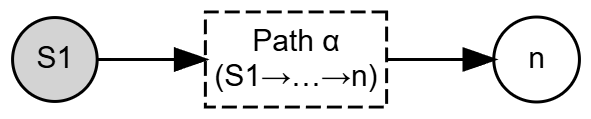
\includegraphics[width=0.55\linewidth]{rId21.png}
\caption{Single-path structure: chained signal propagation.}
\label{fig:chain}
\end{figure}

\begin{figure}[t]
\centering
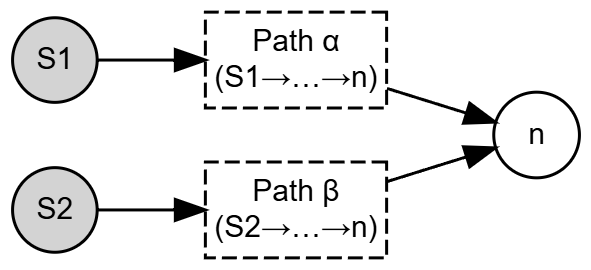
\includegraphics[width=0.55\linewidth]{rId25.png}
\caption{Multiple independent parent signals: parallel signal propagation.}
\label{fig:parallel}
\end{figure}

\subsubsection{Reconvergent Structures and Independence Breakdown}

The update rule in \eqref{eq:independent_update} is no longer exact when the incoming signal events are
dependent. In directed acyclic graphs, this occurs in reconvergent structures, where multiple upstream
paths share common components before merging at a downstream node. Let $v$ be a join node receiving
signals from parents $\{p_1,p_2\}$. If the upstream paths leading to $p_1$ and $p_2$ share a common
ancestor $f$, then the events $A_1$ and $A_2$ are dependent. In that case, applying the
independence-based rule $P(A_1\cup A_2)=1-(1-S_1)(1-S_2)$ overestimates the true probability of signal
reception, because it ignores the correlation induced by the shared upstream components. IPA resolves
this problem by identifying such reconvergent structures and conditioning on the shared upstream
variables that induce the dependency.

\subsubsection{Diamond Structures and Conditional Decomposition}

The fundamental dependency-inducing pattern considered by IPA is a diamond structure: a reconvergent
fork--join subgraph in which multiple paths diverge from one or more shared upstream nodes and
reconverge at a join node. Consider a single-fork diamond with fork node $f$ and join node $j$. Let
$J=\{\text{a signal reaches } j\}$ and $F=\{\text{fork node } f \text{ is reached and operational}\}$.
By the law of total probability,
\begin{equation}\label{eq:diamond_ltp}
P(J)=P(J\mid F)P(F)+P(J\mid \bar F)P(\bar F).
\end{equation}
Conditioning on the state of the fork restores independence among the downstream paths: if $F=1$, the
fork is active and the paths downstream of $f$ become conditionally independent; if $F=0$, no signal can
propagate through paths originating from $f$. Thus, if the diamond contains $k$ downstream paths from
$f$ to $j$, then
\begin{equation}
P(J\mid F)=1-\prod_{i=1}^{k}\bigl(1-S_i(F)\bigr),
\end{equation}
where $S_i(F)$ denotes the probability that path $i$ transmits a signal to $j$ given that the fork is
active. For a simple induced diamond with no alternative upstream routes to the join node,
$P(J\mid \bar F)=0$.

\subsubsection{Generalisation to Multiple Conditioning Nodes}

More complex reconvergent structures may involve several shared upstream nodes
$C=\{c_1,c_2,\dots,c_m\}$. In that case, the join-node signal probability is computed by enumerating all
conditioning states:
\begin{equation}\label{eq:multi_cond}
P(J)=\sum_{s\in\{0,1\}^m} P(J\mid s)\,P(s),
\end{equation}
where $s=(s_1,\dots,s_m)$ is a binary assignment to the conditioning nodes and
\begin{equation}
P(s)=\prod_{i=1}^{m}\bigl[b(c_i)\bigr]^{s_i}\bigl[1-b(c_i)\bigr]^{1-s_i}.
\end{equation}
For each conditioning state $s$, the remaining incoming paths to the join node become conditionally
independent, so the local update can again be evaluated using the independent-signal formula.

\subsection{Simple Example}\label{sec:simple_example}

To illustrate the effect of reconvergent dependencies and the correctness of the conditioning approach,
consider the simple diamond in Figure~\ref{fig:simplediamond}. The subgraph consists of a single
fork--join pair connected by two intermediate paths. All non-source nodes have intrinsic reliability
$0.9$, and all edges have transmission probability $0.9$.

\begin{figure}[t]
\centering
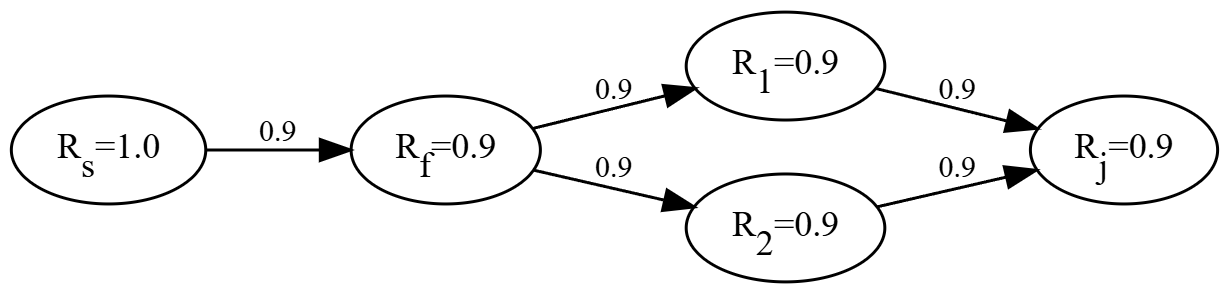
\includegraphics[width=0.7\linewidth]{rId34.png}
\caption{A simple diamond subgraph between fork node $f$ and join node $j$.}
\label{fig:simplediamond}
\end{figure}

\subsubsection{Solution by Path Enumeration (Correct but Expensive)}

We enumerate the relevant fork/intermediate-node states:
\begin{align*}
P_1&=0.81\times0.81\times0.81=0.531441 &&\text{(fork active, both intermediates work)},\\
P_2&=0.81\times0.81\times0.19=0.124659 &&\text{(fork active, only first intermediate works)},\\
P_3&=0.81\times0.19\times0.81=0.124659 &&\text{(fork active, only second intermediate works)},\\
P_4&=0.81\times0.19\times0.19=0.029241 &&\text{(fork active, both intermediates fail)},\\
P_5&=0.19 &&\text{(fork inactive, no signal possible)}.
\end{align*}
The signal-reception probabilities at the join node are $0.99$ if both paths send signals, $0.9$ if only
one path sends a signal, and $0$ if no path sends a signal. Hence,
\begin{align*}
P(\text{signal})&=P_1\times0.99+P_2\times0.9+P_3\times0.9\\
&=0.531441\times0.99+0.124659\times0.9+0.124659\times0.9=0.75051279 .
\end{align*}
The resulting reliability at the join node is
$b(j)=R(j)\,P(\text{signal})=0.9\times0.75051279=0.675461511$.

\subsubsection{Solution by Independent Update (Incorrect)}

Using the independent-parent update yields
\begin{align*}
b(f)&=R(s)\,P(s,f)\,R(f)=1.0\times0.9\times0.9=0.81,\\
b(p_1)=b(p_2)&=b(f)\,P(f,p)\,R(p)=0.81\times0.9\times0.9=0.6561 .
\end{align*}
Thus $S_1=S_2=b(p_i)\,P(p_i,j)=0.6561\times0.9=0.59049$. Treating the two incoming signals as
independent gives
\begin{align*}
P(\text{signal})&=1-(1-0.59049)^2=0.83227,\\
b(j)&=0.9\times0.83227=0.749043,
\end{align*}
which overestimates the correct value.

\subsubsection{Solution by Diamond Conditioning (Correct and Efficient)}

Conditioning on the fork state, we have $b(f)=0.81$. If the fork is active, each downstream path has
conditional transmission probability $P(f,p)\,R(p)\,P(p,j)=0.9\times0.9\times0.9=0.729$. Therefore,
\begin{align*}
P(\text{signal}\mid F=1)&=1-(1-0.729)^2=0.926559, &
P(\text{signal}\mid F=0)&=0 .
\end{align*}
Using \eqref{eq:diamond_ltp},
\begin{align*}
P(\text{signal})&=0.926559\times0.81+0\times0.19=0.75051279 ,
\end{align*}
hence $b(j)=0.9\times0.75051279=0.675461511$, which matches the exact path-enumeration result. This
example shows the central idea behind IPA: the dependence induced by a reconvergent structure can be
handled exactly by conditioning only on the shared upstream variables that generate the dependence.

\subsection{IPA Workflow and Algorithm}\label{sec:workflow}

The Information Propagation Algorithm computes node reliability in a single forward pass over the DAG.
For each node, the algorithm: computes incoming signal probabilities from its parent nodes; applies the
closed-form independent update when the parent signals are independent; detects reconvergent structures
when dependencies are present; and resolves those dependencies through conditional enumeration on shared
upstream nodes. This formulation localises exact dependency handling to the subgraphs that require it,
while retaining simple closed-form updates elsewhere. Algorithm~\ref{alg:ipa} summarises the overall IPA
procedure.

\begin{algorithm}[t]
\caption{Information Propagation Algorithm (IPA)}
\label{alg:ipa}
\begin{algorithmic}[1]
\State Compute a topological ordering of $G$
\For{each node $v$ in topological order}
  \If{$v\in S$} $b(v)\gets R(v)$
  \Else
    \State Compute $S_i=b(p_i)\,P(p_i,v)$ for all $p_i\in\mathrm{Pa}(v)$
    \If{incoming parent signals are independent}
      \State $b(v)\gets R(v)\bigl(1-\prod_i(1-S_i)\bigr)$
    \Else
      \State Identify the reconvergent (diamond) structure affecting $v$
      \State Resolve its dependency by conditional enumeration on the separating set
      \State Compute $b(v)$ from the conditioned signal probabilities
    \EndIf
  \EndIf
\EndFor
\State \Return $\{b(v)\}_{v\in V}$
\end{algorithmic}
\end{algorithm}

\subsubsection{Computational Characteristics}

For nodes with independent parent signals, the update cost is $O(|\mathrm{Pa}(v)|)$, so the total
computational cost is linear in the number of edges for tree-structured networks. For nodes involved in
reconvergent structures, additional cost arises from conditional enumeration over shared upstream
components. If a diamond requires conditioning on $c$ shared upstream variables, the local cost scales
as $O(2^c)$ rather than with the total number of full path combinations. The practical efficiency of IPA
therefore depends primarily on the number and nesting depth of such dependency-inducing structures. The
next section introduces a progressive decomposition strategy that reduces repeated conditioning by
replacing resolved diamond subgraphs with statistically equivalent supernodes.

%% ============================================================================
\section{Progressive Decomposition of Diamond Structures}\label{sec:decomp}

Progressive decomposition is the mechanism that makes IPA practical on many non-trivial DAGs with
reconvergent structure. It preserves exactness by replacing resolved diamonds with conditionally
equivalent supernodes, and it improves efficiency by preventing the same dependencies from being
conditioned on repeatedly.

While conditional decomposition resolves dependencies locally, real process networks rarely contain only
isolated diamonds. In practical directed acyclic graphs, reconvergent structures often overlap or nest
within one another, so that the output of one diamond becomes part of a larger downstream reconvergent
structure. In such cases, repeatedly conditioning on the same upstream variables can lead to severe
computational redundancy. IPA addresses this issue through progressive diamond decomposition. Once a
diamond subgraph has been solved, it is replaced by a statistically equivalent supernode that preserves
its exact conditional behaviour while simplifying the remaining graph.

More generally, for a network with $L$ nested dependency levels, a direct conditional evaluation may
require
\begin{equation}\label{eq:nested_direct_enum}
b(j)=R(j)\!\!\sum_{s_1\in\{0,1\}^{m_1}}\ \sum_{s_2\in\{0,1\}^{m_2}}\!\!\cdots\!\!
\sum_{s_L\in\{0,1\}^{m_L}}\!\! P(s_1)P(s_2\mid s_1)\cdots P(s_L\mid s_1,\dots,s_{L-1})\,
\phi(s_1,\dots,s_L),
\end{equation}
where $m_\ell$ is the number of conditioning nodes introduced at nesting level $\ell$, and $\phi(\cdot)$
is the resulting signal probability at the join node. This cost grows exponentially with both the number
of conditioning variables and the depth of nesting. The purpose of progressive decomposition is to avoid
this repeated re-evaluation by solving inner diamonds once, storing their exact conditional behaviour,
and reusing that information whenever the reduced network is evaluated further downstream.

\subsection{Supernode Representation and Exactness Guarantees}\label{sec:supernode}

Let $D$ be a diamond subgraph with fork-side conditioning set $C_D=\{c_1,\dots,c_m\}$ and join node
$j_D$. Solving the diamond yields the exact conditional signal probability at the join node for every
configuration of the conditioning variables:
\begin{equation}\label{eq:supernode_conditional_map}
\psi_D(s)=P(J_D\mid s), \qquad s\in\{0,1\}^m,
\end{equation}
where $J_D$ denotes the event that a signal reaches the join node of the diamond and $s$ is a binary
state assignment to $C_D$. The resolved diamond is then replaced by a supernode that stores the map
$s\mapsto\psi_D(s)$. This supernode acts as a statistically equivalent component in the reduced graph:
whenever the conditioning state $s$ is encountered in a larger downstream computation, the contribution
of the original diamond is recovered exactly through \eqref{eq:supernode_conditional_map}, without
re-solving the full subgraph. The following lemmas make the exactness guarantees precise.

\begin{lemma}[Conditional invariance]\label{lem:invariance}
Let $A\subseteq V$ and let $\mathcal{R}_A$ denote the vector of reachability indicators of $A$. Then for
any node $v$,
\begin{equation}\label{eq:ltp}
b(v)=\sum_{c\in\{0,1\}^{|A|}} P(\mathcal{R}_A=c)\; P(\mathcal{R}_v=1\mid \mathcal{R}_A=c),
\end{equation}
and the decomposition is well defined because every $\mathcal{R}_u$ is a deterministic function of the
mutually independent component indicators $\{X_w, X_{wu}\}$. Moreover, let $D$ be a diamond subgraph with
join $j$ and conditioning set $C\subseteq F\cap\mathrm{anc}(j)$, and let
$\psi_D(c)=P(J_D\mid \mathcal{R}_C=c)$ denote its conditional signal map. If an enclosing computation
conditions on further variables $A'$ with $A'\cap D=\emptyset$ --- that is, the outer conditioning fixes
no variable internal to $D$ --- then $\psi_D(c)$ is unchanged: outer conditioning affects only the
weights $P(\mathcal{R}_C=c\mid \mathcal{R}_{A'})$, never the map $\psi_D$ itself.
\end{lemma}

\begin{proof}
The first display is the law of total probability over the partition $\{\mathcal{R}_A=c\}$. For the
second claim, fix $c$. Conditional on $\mathcal{R}_C=c$, the event $J_D$ is determined by the indicators
of nodes and edges internal to $D$. By Assumption~\ref{as:indep} these are independent of every indicator
outside $D$, hence of $\mathcal{R}_{A'}$ whenever $A'$ contains no internal variable of $D$.
Consequently $P(J_D\mid \mathcal{R}_C=c,\mathcal{R}_{A'}=a)=P(J_D\mid \mathcal{R}_C=c)$ for every outer
state $a$.
\end{proof}

The condition $A'\cap D=\emptyset$ is essential and is enforced by the identification procedure: when an
outer conditioning does fix a variable internal to a previously resolved subgraph --- as can occur when
diamonds overlap or share conditioning nodes --- the sub-problem is a different one and is resolved (and
stored) separately under its own conditioning context. Section~\ref{sec:identification} makes this
identification precise. A conditioning variable already fixed by an outer state contributes a single
term to the enumeration rather than two, so overlapping conditioning never doubles work unnecessarily.

\begin{lemma}[Separator sufficiency]\label{lem:separator}
Let $v$ be a join node with parents $\mathrm{Pa}(v)$, and let $C\subseteq F\cap\mathrm{anc}(v)$ be such
that every directed path from a common ancestor of two distinct parents $u_i,u_j\in\mathrm{Pa}(v)$ to
those parents intersects $C$ --- that is, $C$ is a cutset of the parents' shared ancestry. Then,
conditional on $\mathcal{R}_C$, the parent reachability events $\{\mathcal{R}_{u_i}\}$ are mutually
independent, and
\begin{equation}
b(v\mid \mathcal{R}_C=c)=R(v)\left(1-\prod_{u\in\mathrm{Pa}(v)}
\bigl(1-P(\mathcal{R}_u=1\mid \mathcal{R}_C=c)\,P(u,v)\bigr)\right).
\end{equation}
\end{lemma}

\begin{proof}
With $\mathcal{R}_C$ fixed, the residual ancestries $\mathrm{infl}(u_i;C)$ of distinct parents share no
component indicator, by the cutset property. Each $\mathcal{R}_{u_i}$, conditional on $\mathcal{R}_C$,
is a function of its residual ancestry alone; functions of disjoint sets of independent variables are
independent. The display is then the independent-union rule \eqref{eq:independent_update} applied
conditionally.
\end{proof}

Lemma~\ref{lem:separator} is the justification for the conditioning sets used throughout: the
identification procedure returns, for each reconvergent structure, a separating set $C$ satisfying the
cutset property, and the per-structure cost $2^{|C|}$ follows.

\begin{lemma}[Independent-substructure factorisation]\label{lem:factorisation}
Fix a conditioning context $E_c$ and, for parents $u,u'$ of a join $v$, write $u\sim u'$ whenever
$\mathrm{infl}(u;E_c)\cap\mathrm{infl}(u';E_c)\neq\emptyset$. Let $G_1,\dots,G_m$ be the equivalence
classes of $\mathrm{Pa}(v)$ under the transitive closure of $\sim$. Then the events
$\{v \text{ is reached through some parent in } G_k\}$, $k=1,\dots,m$, are mutually independent, so
\begin{equation}
b(v)=R(v)\left(1-\prod_{k=1}^{m}\bigl(1-P(v \text{ reached via } G_k)\bigr)\right),
\end{equation}
and each class $G_k$ can be conditioned on its own separating set $C_k$ independently of the others.
\end{lemma}

\begin{proof}
Distinct classes have disjoint unresolved influence by construction, so the class events are functions of
disjoint sets of independent indicators, hence independent; the product form is the union rule for
independent events.
\end{proof}

The practical effect is substantial. At a join whose $k$ parents share ancestry only pairwise within $m$
independent groups, joint conditioning would enumerate $2^{|C_1|+\cdots+|C_m|}$ states, whereas
factorised conditioning enumerates $\sum_k 2^{|C_k|}$. In the extreme case of $k$ parents each depending
on its own single fork, the cost falls from $2^k$ to $2k$ --- from exponential to linear in the fan-in.

\begin{lemma}[Supernode equivalence]\label{lem:supernode}
Let $D$ be a resolved diamond with conditional signal map $\psi_D(s)$. Replacing $D$ by a supernode
storing $\psi_D(s)$ preserves the exact source-to-node reliability of every downstream node in the
reduced graph.
\end{lemma}

\begin{proof}
For any downstream computation, the contribution of $D$ enters only through the probability that its
join node receives a signal under a given conditioning state. By Lemma~\ref{lem:invariance} the stored
map $\psi_D(c)$ equals $P(J_D\mid \mathcal{R}_C=c)$ in every outer context that fixes no internal
variable of $D$, and by Lemma~\ref{lem:separator} the downstream update uses only these conditional
probabilities together with the weights $P(\mathcal{R}_C=c)$; both are preserved by the replacement, so
every downstream belief is unchanged.
\end{proof}

\subsection{Progressive Decomposition Procedure}\label{sec:procedure}

IPA applies diamond decomposition progressively during topological evaluation. When the algorithm
reaches a join node involved in a reconvergent structure, it: identifies the associated diamond
subgraph; determines the conditioning variables required to resolve its internal dependencies; computes
the conditional signal map of the join node; and replaces the entire resolved diamond by a supernode in
the reduced graph. This procedure transforms the original DAG into a progressively simpler equivalent
DAG. Inner diamonds are resolved first, so that larger outer diamonds can treat them as supernodes
rather than re-evaluating their internal paths. Figure~\ref{fig:decomposition} illustrates the
decomposition of a nested reconvergent network.

\begin{figure}[p]
\centering
\begin{subfigure}[b]{0.48\linewidth}
  \centering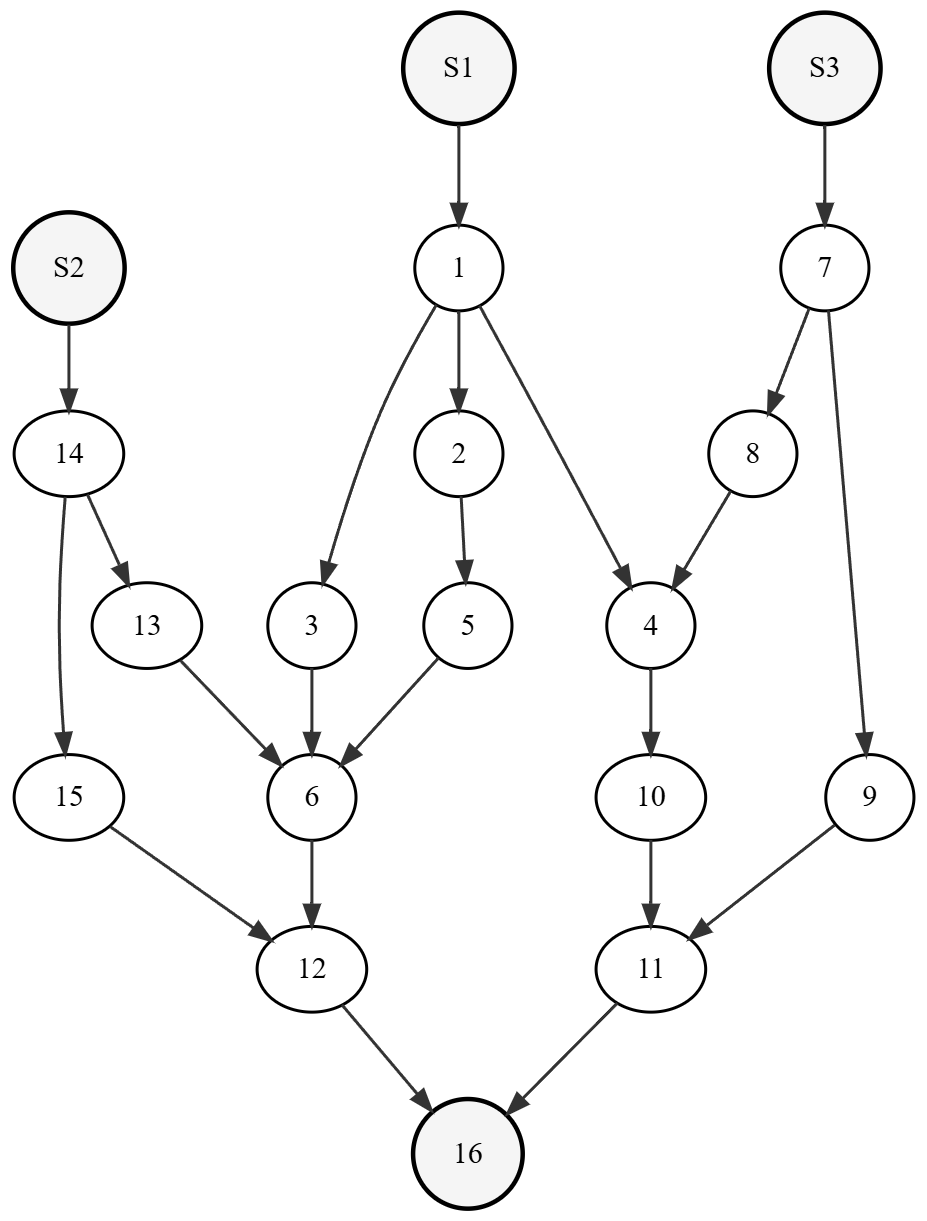
\includegraphics[height=0.26\textheight,keepaspectratio]{rId46.png}
  \caption{Original network}
\end{subfigure}\hfill
\begin{subfigure}[b]{0.48\linewidth}
  \centering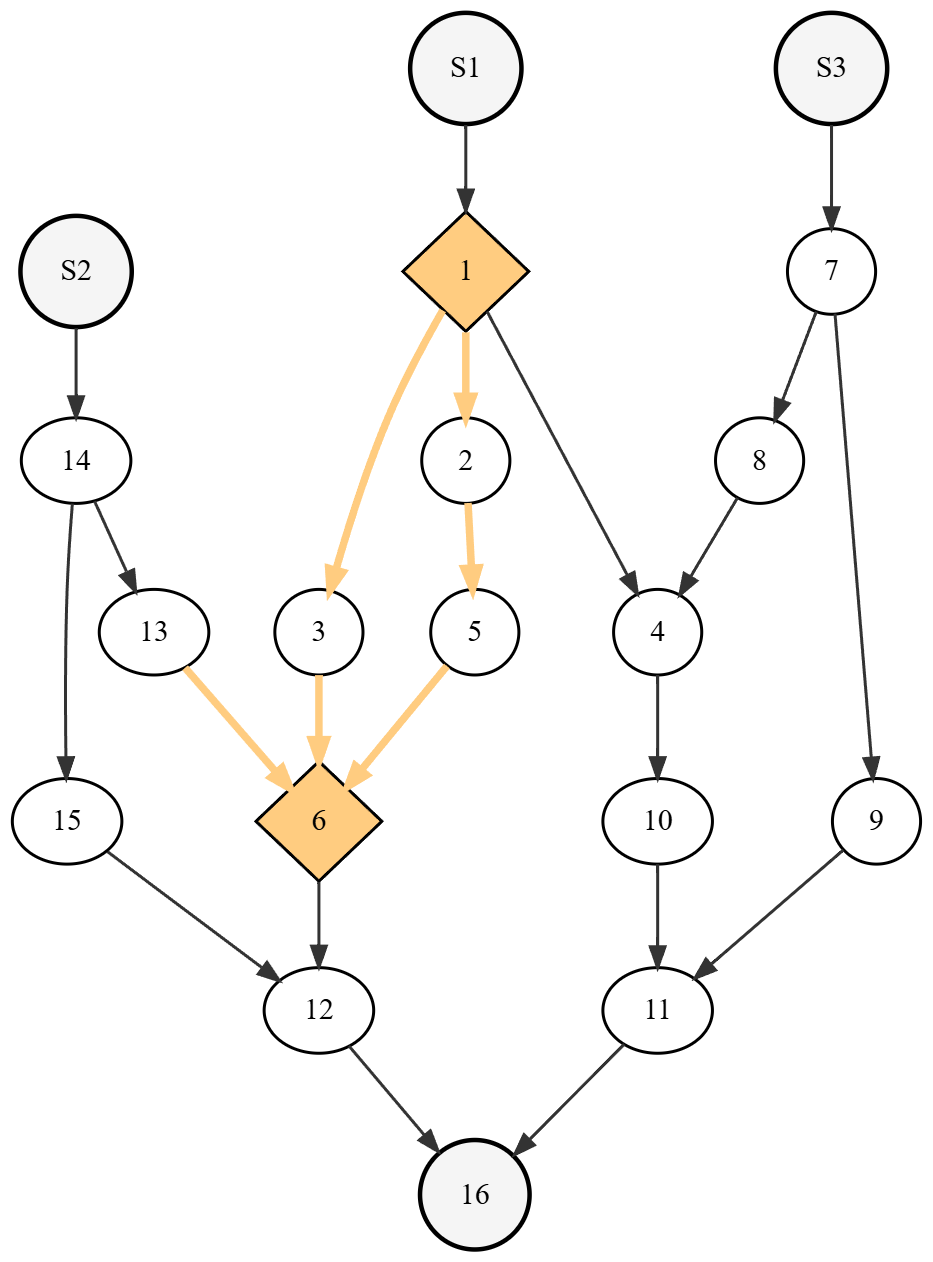
\includegraphics[height=0.26\textheight,keepaspectratio]{rId50.png}
  \caption{Diamond $D_1$: $1\to6$}
\end{subfigure}\\[2mm]
\begin{subfigure}[b]{0.48\linewidth}
  \centering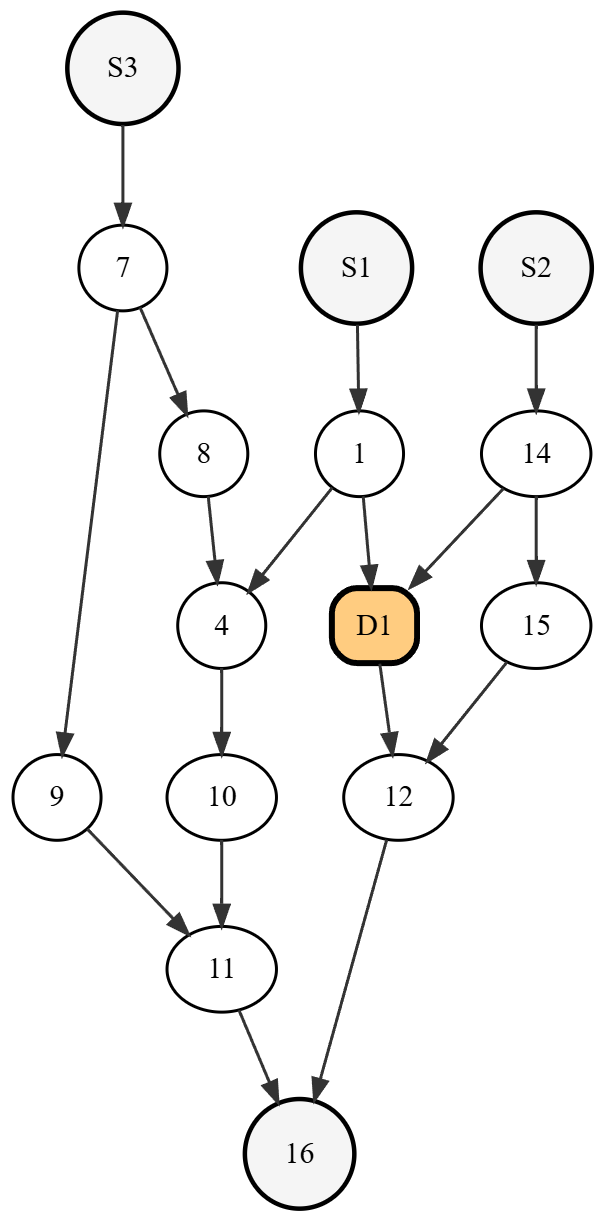
\includegraphics[height=0.26\textheight,keepaspectratio]{rId54.png}
  \caption{After $D_1$ replacement}
\end{subfigure}\hfill
\begin{subfigure}[b]{0.48\linewidth}
  \centering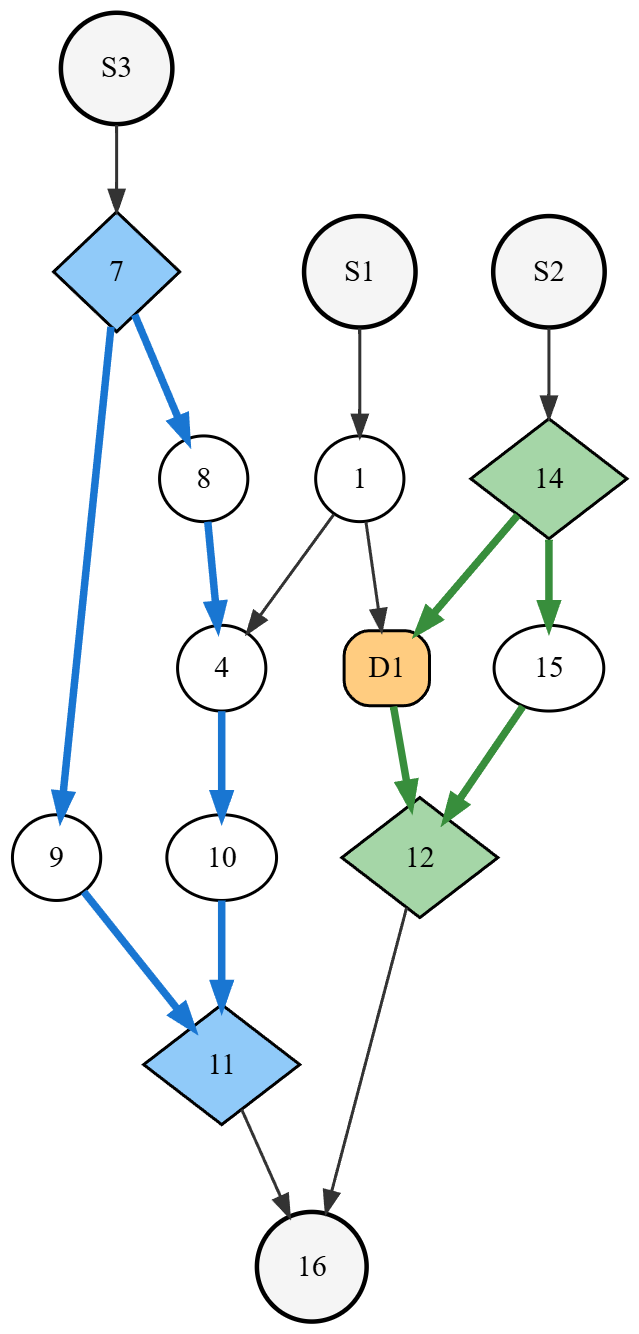
\includegraphics[height=0.26\textheight,keepaspectratio]{rId58.png}
  \caption{Diamonds $D_2$: $7\to11$, $D_3$: $14\to12$}
\end{subfigure}\\[2mm]
\begin{subfigure}[b]{0.31\linewidth}
  \centering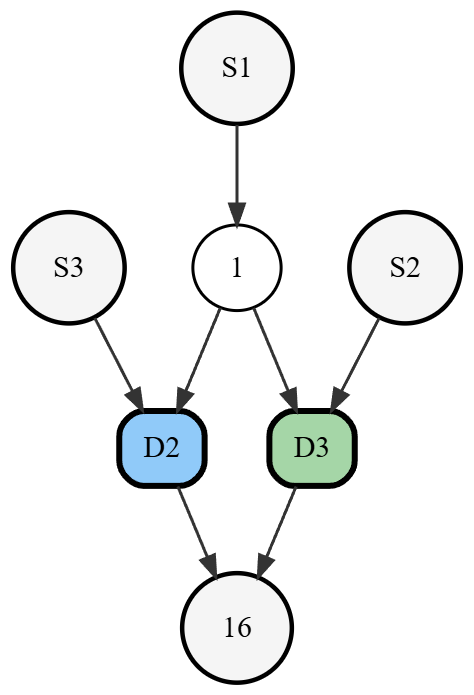
\includegraphics[height=0.24\textheight,keepaspectratio,width=\linewidth]{rId62.png}
  \caption{After $D_2$, $D_3$ replacement}
\end{subfigure}\hfill
\begin{subfigure}[b]{0.31\linewidth}
  \centering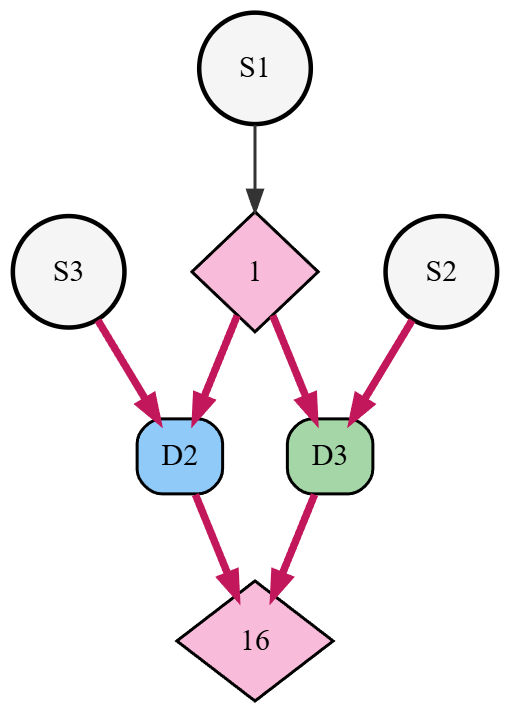
\includegraphics[height=0.24\textheight,keepaspectratio,width=\linewidth]{rId66.png}
  \caption{Final diamond $D_4$: $1\to16$}
\end{subfigure}\hfill
\begin{subfigure}[b]{0.31\linewidth}
  \centering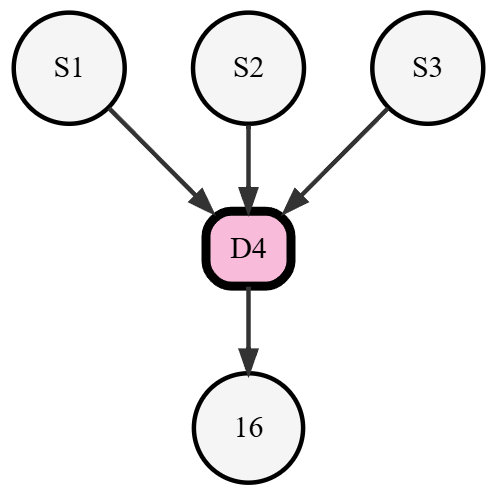
\includegraphics[height=0.24\textheight,keepaspectratio,width=\linewidth]{rId70.png}
  \caption{Final decomposition}
\end{subfigure}
\caption{Progressive diamond decomposition in a nested reconvergent network.}
\label{fig:decomposition}
\end{figure}

The topological order ensures that the inner diamond $D_1$ is detected and resolved before downstream
join nodes are processed. Once replaced by a supernode, the reduced graph contains fewer explicit
dependency-inducing paths. The same procedure is then applied to $D_2$ and $D_3$, after which the final
outer diamond $D_4$ can be evaluated using the already-resolved supernodes. In this way, dependencies are
handled locally and only once.

\subsubsection{Worked multi-level example}\label{sec:worked}

To make the procedure concrete, consider the network of Figure~\ref{fig:decomposition} with all
non-source nodes assigned intrinsic reliability $0.9$, all edges transmission probability $0.9$, and
source reliabilities $1.0$. Table~\ref{tab:trace} traces the four diamond resolutions: for each, the
fork whose reachability is conditioned on, the weight $w=P(\mathcal{R}_f=1)$, the two conditional signal
maps, and the resulting belief at the join node. The inner diamond $D_1$ (fork $1$, join $6$) is
resolved by enumerating the two states of its fork; note that its join retains a nonzero conditional
value when the fork is down, because the path from source $S_2$ through node $13$ is unaffected by the
fork. $D_2$ and $D_3$ are resolved in the same way. The outer diamond $D_4$ (fork $1$, join $16$) then
conditions on the same fork; within each of its two states, the nested structures at joins $6$, $11$,
and $12$ are required under that outer context and are supplied by their stored conditional maps ---
re-resolved only where the outer state changes their context (Section~\ref{sec:identification}), for
example $b(12\mid \mathcal{R}_1{=}1)=0.8098$ versus $b(12\mid \mathcal{R}_1{=}0)=0.6481$.

\begin{table}[t]
\centering\small
\caption{Trace of the worked multi-level example (Figure~\ref{fig:decomposition}): the four diamond
resolutions in their base context. $w=P(\mathcal{R}_f=1)$; $\psi(1),\psi(0)$ are the conditional signal
probabilities at the join given the fork reachable/unreachable.}
\label{tab:trace}
\begin{tabular}{lcccccc}
\toprule
Diamond & Join $j$ & Fork $f$ & $w$ & $\psi(1)$ & $\psi(0)$ & $b(j)=w\,\psi(1)+(1{-}w)\,\psi(0)$\\
\midrule
$D_1$ & 6  & 1  & 0.81 & 0.85910 & 0.53144 & 0.79684\\
$D_2$ & 11 & 7  & 0.81 & 0.80437 & 0.43047 & 0.73333\\
$D_3$ & 12 & 14 & 0.81 & 0.83867 & 0.52496 & 0.77907\\
$D_4$ & 16 & 1  & 0.81 & 0.82255 & 0.73623 & 0.80615\\
\bottomrule
\end{tabular}
\end{table}

The final belief at node $16$ is $b(16)=0.80614907$, and every node's belief agrees with exhaustive path
enumeration (inclusion--exclusion over all source-to-node paths) to within $3.4\times10^{-16}$, i.e.\
floating-point round-off. The effect of reuse is also measurable on this small example: resolving the
network requires the evaluation of $68$ distinct conditional sub-problems with supernode reuse, against
$145$ evaluations if every nested structure is re-evaluated in every context in which it appears.

\subsubsection{Identification of stored sub-problems}\label{sec:identification}

A resolved sub-structure is identified by the pair (induced substructure, conditioning context): the
internal nodes and edges of the diamond together with the set of upstream variables whose states are
fixed when it is resolved. Two occurrences of the same substructure reached under different conditioning
contexts are treated as distinct sub-problems, because an outer state that fixes a variable inside the
substructure changes its conditional signal map (cf.\ the condition of Lemma~\ref{lem:invariance}). This
context-aware identification is what guarantees correctness when diamonds overlap or share conditioning
variables: reuse occurs only between genuinely identical sub-problems. Conversely, a conditioning
variable whose state is already determined by the enclosing enumeration contributes a single state rather
than two, so the enumeration never expands over variables that carry no remaining uncertainty. Together
these two rules bound the stored state space by the number of genuinely distinct conditional
sub-problems, which is the quantity reported as realised computational work in
Section~\ref{sec:comparison}.

\subsection{Complexity and Relation to Established Exact Methods}\label{sec:complexity}

The computational cost of the procedure admits an exact per-instance expression. Let the recursion of
Section~\ref{sec:procedure} resolve diamonds $d=1,\dots,M$ (counting nested resolutions), with
conditioning sets $C_d$ and internal edge sets $E_d$. The work performed is
\begin{equation}\label{eq:work}
W=\sum_{d=1}^{M} 2^{|C_d|}\cdot O(|E_d|),
\end{equation}
since each diamond is resolved by enumerating the $2^{|C_d|}$ states of its conditioning set and each
state requires a propagation over the diamond's internal structure. Every term of this sum is available
before enumeration begins, because the conditioning sets are produced by the identification procedure
itself; $W$ is therefore a sound a-priori \emph{upper bound} on the cost of an analysis, computable in
advance for a given network, rather than merely an asymptotic bound. It is an upper bound rather than the
realised cost because memoisation of resolved sub-problems (Section~\ref{sec:identification}) reduces
the work actually performed to the number of genuinely distinct conditional sub-problems encountered ---
observed to be a small fraction of $W$ in practice --- which is the quantity measured in the experiments
below. The factorisation of Lemma~\ref{lem:factorisation} reduces
the exponents themselves in favourable cases --- at a fan-in of $k$ independent branches, from $2^k$
states to a number linear in $k$ --- without changing the worst-case class.

\paragraph{Relation to cutset conditioning and junction trees}
The procedure is a specialisation of cutset conditioning (Pearl 1988) to source-to-node reachability in
DAGs. Classical cutset conditioning selects a single global cutset whose state enumeration renders the
whole network singly connected, at cost exponential in the cutset size; the present method instead
identifies, at each reconvergence actually encountered, a local separating set of the parents' shared
ancestry (Lemma~\ref{lem:separator}), conditions on it, and recurses, so that the realised cost is a sum
of local exponentials rather than one global exponential. Tree-structured regions of the network are
traversed by the closed-form updates of Section~\ref{sec:ipa} at linear cost, and the factorisation of
Lemma~\ref{lem:factorisation} prevents joint conditioning over forks that are independent given the
current context. The maximum conditioning-set size encountered on a network is bounded by the size of
the largest set of mutually entangled shared ancestors, a quantity that is in turn bounded by --- and,
as shown below, empirically tracks --- the treewidth of the network. The method therefore sits in the
same parametric complexity class as the junction-tree algorithm (cost exponential in treewidth;
Lauritzen and Spiegelhalter 1988) and as a well-ordered reduced binary decision diagram (size
exponential in pathwidth): all are exact, all are fixed-parameter tractable in the relevant width, and
none escapes the \#P-hardness of the underlying problem. No closed-form complexity in the node count
alone exists for any of them.

\paragraph{Measured comparison}
Section~\ref{sec:comparison} reports, for every network in the validation corpus, the maximum
conditioning-set size, the realised number of conditional sub-problems, and the node count of a
reduced-ordered binary decision diagram for the same network built under dynamic variable reordering.
Two findings anticipate the details. First, the maximum conditioning-set size sits in the same band as
the logarithm of the decision-diagram size --- for example $7$ against $8.2$ on a $4{\times}4$ grid,
$10$ against $9.0$ on a bridge network, $13$ against $11.7$ on the densest random network tested
(Figure~\ref{fig:width}) --- confirming that both methods are governed by the same structural width
parameter. Second, the realised work of the proposed method is of the same order as the decision-diagram
size, sometimes smaller and sometimes larger, with neither method dominating across the corpus. We state
the conclusion plainly: for exact point-valued reliability the proposed method is competitive with, but
not structurally superior to, a well-ordered decision diagram. Its distinguishing capability lies in the
native propagation of imprecise component reliabilities (Section~\ref{sec:imprecise}), which
decision-diagram methods do not provide.

\subsection{Numerical Realisation}\label{sec:numerical}

The propagation scheme of Sections~\ref{sec:ipa}--\ref{sec:decomp} is arithmetic over the operations
$\{+,\times,\text{complement}\}$ on component reliabilities, and is realised once, generically, for the
three input forms of Section~\ref{sec:imprecise_model}: point values, intervals, and probability boxes.
Three numerical points warrant note. First, multi-parent updates are evaluated in the product form
$1-\prod_i(1-p_i)$ rather than by the alternating inclusion--exclusion sum; the two are equivalent under
independence, but the product form is numerically stable and, for interval-valued inputs, avoids the
spurious widening that alternating sums introduce. Second, for interval inputs the conditioning step is
evaluated at the corner states of the conditioning bounds and the result enclosed in an interval
envelope; Section~\ref{sec:interval} shows this yields the exact range, by monotonicity. Third, for
p-box inputs the conditioning recombination at a join is a convex combination of two dependent random
quantities, not an independent sum; it is evaluated by the operator of Section~\ref{sec:pbox}, which
integrates over the distribution of the conditioning weight and bounds the branch dependence by the
Fr\'echet--Hoeffding inequalities. Because the underlying floating-point arithmetic is not
outward-rounded, the computed bounds are intersected with $[0,1]$ as a final step --- a projection that
can only tighten a bound on a probability, never invalidate it --- and this projection is guarded: an
excursion beyond $[0,1]$ exceeding ordinary floating-point round-off by several orders of magnitude
raises an error rather than being silently discarded, so that a genuine soundness regression cannot be
masked as rounding. The full implementation, together with all validation scripts and data, is openly
available (see Data and Software Availability).

%% ============================================================================
\section{Case Studies}\label{sec:cases}

This section evaluates IPA in four steps: a benchmark validation on a grid network
(Section~\ref{sec:grid}); a corpus-wide validation and cost comparison against an independent exact
decision-diagram method (Section~\ref{sec:comparison}); the imprecise-propagation capability
(Section~\ref{sec:imprecise}); and an applied reliability case study of a medical drone logistics
network for Scotland (Section~\ref{sec:drone}). All runtimes reported in this section were measured
after a warm-up run of the same computation was executed and discarded, so that one-off
program-initialisation cost is excluded from every figure; each reported time is the minimum of repeated
measurements on otherwise idle hardware. All decision-diagram comparisons use CUDD, called from the same
process and the same machine as the proposed method, with dynamic variable reordering enabled unless
stated otherwise. Where component reliabilities are widened into intervals or probability boxes for
illustration, this widening is applied only to components that are not structurally certain: a component
fixed at reliability exactly 0 or 1 by the network's own structure (for example, a supply hub assumed
always available) is left exactly at that value rather than being given synthetic uncertainty, since
degrading a structural certainty into an uncertain quantity changes the problem being analysed rather
than merely adding noise to it.

\subsection{Benchmark Validation on a Grid Network}\label{sec:grid}

\subsubsection{Benchmark setup}

Both the proposed Information Propagation Algorithm and Tong and Tien's directed Probability Propagation
Method (dPrPm) (Tong and Tien 2019) compute node reliability in directed acyclic networks by propagating
local probability information from upstream to downstream nodes. Both methods exploit the acyclic
structure of the graph to ensure that upstream dependencies are processed before downstream updates. The
two methods differ in how dependencies are represented and resolved. dPrPm propagates both marginal and
pairwise probabilities and uses local approximations to account for dependent interactions.
Specifically, when multiple predecessors influence a node, the update rules explicitly rely on
approximating a three-node joint distribution for every new edge introduced. Although effective, this
approach requires storing both marginal and pairwise probabilities throughout the network, which can
become memory-intensive in large or dense networks. IPA takes a fundamentally different view of network
dependencies: it identifies reconvergent dependency patterns as diamond structures and resolves them
through conditional decomposition. Rather than tracking pairwise relationships, it decomposes these
structures into statistically equivalent supernodes, so the relevant dependency structure is captured
inherently in the decomposition.

To provide a direct benchmark, IPA is applied to the same 16-node directed grid network studied in Tong
and Tien (2019), shown in Figure~\ref{fig:grid}. This benchmark is useful because it contains multiple
reconvergent structures while remaining small enough for exact verification by explicit path-based
computation. Following the source study, all source nodes are assigned prior reliability $1.0$ and all
directed edges are assigned transmission probability $0.9$.

\begin{figure}[t]
\centering
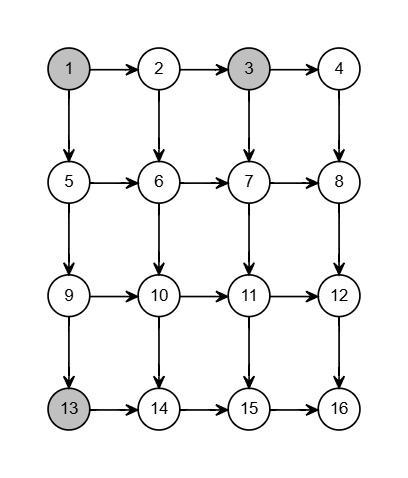
\includegraphics[width=0.5\linewidth]{rId80.png}
\caption{16-node directed grid network (Tong and Tien 2019). Source nodes 1, 3, and 13 are coloured in
grey.}
\label{fig:grid}
\end{figure}

\subsubsection{Accuracy results}

Table~\ref{tab:grid_accuracy} compares the node reliabilities obtained using IPA with exact values and
with the lower and upper bounds reported for dPrPm in Tong and Tien (2019). IPA reproduces the exact
values up to floating-point precision. By contrast, dPrPm provides tight lower and upper bounds that
coincide with the exact values for many nodes in this benchmark.

\begin{table}[t]
\centering\small
\caption{Node reliabilities on the benchmark grid network at link reliability $R_l=0.9$. IPA reproduces
the exact values at every node to floating-point precision; dPrPm lower/upper bounds and gap are as
reported in Tong and Tien (2019, Table~2). Source nodes (1, 3, 13) are fixed at reliability 1 and are
not reported as dPrPm bounds in the source study.}
\label{tab:grid_accuracy}
\begin{tabular}{ccccc}
\toprule
Node & Exact = IPA & dPrPm lower & dPrPm upper & Gap\\
\midrule
1  & 1.0        & --      & --      & --\\
2  & 0.99000000 & 0.99000 & 0.99000 & 0.00000\\
3  & 1.0        & --      & --      & --\\
4  & 0.98015430 & 0.98015 & 0.98015 & 0.00000\\
5  & 0.90000000 & 0.90000 & 0.90000 & 0.00000\\
6  & 0.99510274 & 0.99510 & 0.99510 & 0.00000\\
7  & 0.98955925 & 0.98956 & 0.98956 & 0.00000\\
8  & 0.89060332 & 0.89060 & 0.89060 & 0.00000\\
9  & 0.98100000 & 0.98100 & 0.98100 & 0.00000\\
10 & 0.88290000 & 0.88290 & 0.88290 & 0.00000\\
11 & 0.97734390 & 0.97734 & 0.97734 & 0.00000\\
12 & 0.97456525 & 0.97457 & 0.97457 & 0.00000\\
13 & 1.0        & --      & --      & --\\
14 & 0.97946100 & 0.97946 & 0.97946 & 0.00000\\
15 & 0.98497989 & 0.98498 & 0.98498 & 0.00000\\
16 & 0.98538853 & 0.98506 & 0.98558 & 0.00048\\
\bottomrule
\end{tabular}
\end{table}

The dPrPm bounds coincide with the exact solution, to the precision reported by the source study, at
every node except node 16, where a gap of $0.00048$ remains --- the same node the source study itself
identifies as the lowest-probability, hardest-to-bound event in this benchmark. IPA carries no such gap
at any node.

Table~\ref{tab:grid_runtime} reports the runtime of IPA on the benchmark network alongside the runtime
reported for dPrPm in Tong and Tien (2019). Two caveats attend this comparison and we state them
plainly. First, the dPrPm figure is quoted from the source study and was obtained in a different
implementation environment; the comparison is indicative only, and no controlled speed claim is based on
it. Second, the dPrPm reference implementation is not publicly available and its authors could not be
reached, so the comparison cannot be reproduced independently. For these reasons the quantitative
performance assessment of the proposed method in this paper rests on the controlled, same-environment
comparison against an independent exact method in Section~\ref{sec:comparison}, and dPrPm is retained
only as the published point of reference that motivated the benchmark.

\begin{table}[t]
\centering\small
\caption{Computational performance on the benchmark grid network. IPA figures are machine-specific
(measured on the authors' current hardware after a discarded warm-up run) and are reported to
characterise order of magnitude, not for cross-machine comparison. The dPrPm runtime is quoted from Tong
and Tien (2019) and is indicative only (different implementation environment; memory data not
available).}
\label{tab:grid_runtime}
\begin{tabular}{lcc}
\toprule
Method & Runtime & Memory\\
\midrule
IPA & 0.928\,ms & 1.72\,MB\\
dPrPm (reported) & 0.32\,s & n/a\\
\bottomrule
\end{tabular}
\end{table}

The benchmark has also been re-verified independently. The node reliabilities produced by the proposed
method were compared against a reduced-ordered binary decision diagram with dynamic variable reordering
--- a canonical independent exact method --- constructed for the same network; the worst per-node
disagreement is $1.1\times10^{-16}$, i.e.\ floating-point round-off, confirming the values in
Table~\ref{tab:grid_accuracy}. During this hardening the diamond-identification procedure was also
stress-tested beyond the benchmark's parameterisation (non-unit node priors, and the boundary case in
which all node priors equal one); two edge-case identification errors were found and corrected, and the
corrected procedure is the one validated across the full corpus of Section~\ref{sec:comparison}. Neither
error affects the benchmark table, which stands as originally reported.

\subsection{Validation and Cost Comparison Against an Exact Decision-Diagram Method}\label{sec:comparison}

To address the breadth of validation, the proposed method was compared against an independent exact
method --- a reduced-ordered binary decision diagram (ROBDD) with dynamic variable reordering --- across
a corpus of 129 random and mutated DAGs (10 to 28 nodes, densities 0.14--0.42), six topological families
(multi-source, grid/lattice, layered, bridge, series--parallel, complete), larger random networks up to
50 nodes, and several real infrastructure networks: a gas distribution network (Memphis Light, Gas and
Water), a metropolitan transit network (Berlin), and a water distribution benchmark (EPANET Net3), in
addition to the power distribution and drone logistics networks studied in detail below. Every network in
the corpus was evaluated by both methods; the worst per-node disagreement observed anywhere is
$1.1\times10^{-16}$, for both perfect and imperfect component reliabilities. Structural exactness was
additionally verified against 17 published Bayesian-network benchmark topologies (bnlearn.com/bnrepository),
ranging from 8 to 1{,}041 nodes; component reliabilities on these networks are illustrative rather than
decision-relevant, and the exercise is intended to demonstrate breadth of topology and scale rather than
to make a claim about any of the systems the benchmarks originally model. Table~\ref{tab:corpus} summarises
the random corpus and Table~\ref{tab:structured} reports representative structured and real networks in
detail.

\begin{table}[t]
\centering\small
\caption{Exactness and complexity of IPA on named structured networks, versus the exact ROBDD oracle.
\emph{root D./uniq.\ D.} are the numbers of root and unique diamond structures identified;
$\max|C|$ is the largest conditioning set; \emph{ROBDD} is the node count under dynamic reordering;
$\max|\Delta|$ is the worst per-node deviation of IPA from the exact ROBDD reliability.}
\label{tab:structured}
\begin{tabular}{lrrrrrrrl}
\toprule
Network & $|V|$ & $|E|$ & src & root D. & uniq.\ D. & $\max|C|$ & ROBDD & $\max|\Delta|$\\
\midrule
power network      & 23 & 27 & 3 &  5 &   9 &  3 &  384 & $8.3\times10^{-17}$\\
grid (benchmark)   & 16 & 24 & 3 &  8 &  39 &  7 &  290 & $1.1\times10^{-16}$\\
Karl network       & 26 & 74 & 1 & 18 & 145 & 11 & 1921 & $5.6\times10^{-17}$\\
counterexample-n15 & 15 & 23 & 1 &  4 &  13 &  4 &  340 & $5.6\times10^{-17}$\\
\bottomrule
\end{tabular}
\end{table}

\begin{table}[t]
\centering\small
\caption{Random and mutated DAG corpus (129 unique graphs), summarised by family. Random DAGs are
generated per family with edge probability $p\in\{0.10,0.15,0.20\}$ and eight seeds; \emph{mutant-n28}
is a base $n{=}28$ DAG with $+5/-2$ edge mutations. Every graph in every family was validated exact
against the ROBDD oracle ($\max|\Delta|\le1.1\times10^{-16}$ across the whole corpus).
\emph{Naive blow-ups} are builds exceeding $2.5\times10^{6}$ ROBDD nodes under a naive (topological)
variable order, all of which dynamic reordering resolves.}
\label{tab:corpus}
\begin{tabular}{lrrrrrrr}
\toprule
Family & \#graphs & $|V|$ & $|E|$ & density & med.\ ROBDD & max.\ ROBDD & naive blow-ups\\
\midrule
random-n10  & 24 & 10 & 12--18 & 0.27--0.40 &   80 &   270 & 0\\
random-n12  & 24 & 12 & 15--28 & 0.23--0.42 &  197 &   693 & 0\\
random-n15  & 24 & 15 & 21--35 & 0.20--0.33 &  450 &  1092 & 0\\
random-n20  & 24 & 20 & 31--50 & 0.16--0.26 & 1164 &  2849 & 0\\
random-n25  & 24 & 25 & 42--73 & 0.14--0.24 & 3119 & 20323 & 9\\
mutant-n28  &  8 & 28 & 62     & 0.16       & 2562 &  6050 & 6\\
counterexample & 1 & 15 & 23   & 0.22       &  340 &   340 & 0\\
\bottomrule
\end{tabular}
\end{table}

The comparison also quantifies cost. For each network we report the maximum conditioning-set size
$|C|_{\max}$ encountered by the proposed method, its realised number of distinct conditional
sub-problems, and the ROBDD node count under dynamic reordering. As anticipated in
Section~\ref{sec:complexity}, $|C|_{\max}$ tracks the logarithm of the ROBDD size across the corpus
(Figure~\ref{fig:width}) --- the two methods are governed by the same structural width --- and the
realised work of the two methods is of the same order, with neither dominating: on some networks the
proposed method resolves fewer sub-problems than the diagram has nodes (e.g.\ 42 against 340 on the
counterexample network; 142 against 759 on the complete 8-node network), on others more (e.g.\ 1961
against 1043 on a layered network). No family in the corpus favours the proposed method for exact
point-valued computation. This is an honest structural finding, and it sharpens rather than weakens the
contribution: the value of the proposed method rests on the capabilities of
Section~\ref{sec:imprecise}, not on a claim of a smaller exact state space.

\begin{figure}[t]
\centering
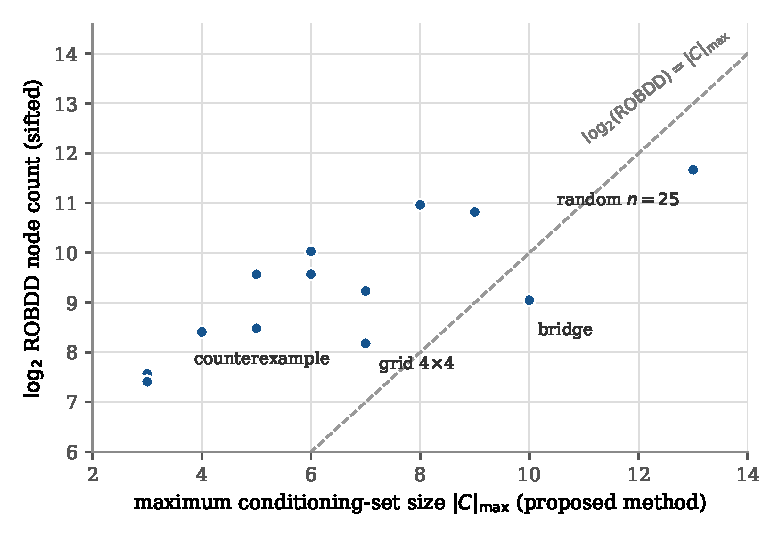
\includegraphics[width=0.75\linewidth]{width_correlation.pdf}
\caption{The proposed method's maximum conditioning-set size against the logarithm of the sifted ROBDD
node count, across the complexity-validation networks. Both quantities measure the same structural width
of the network; neither method dominates.}
\label{fig:width}
\end{figure}

\subsection{Imprecise Reliability Propagation}\label{sec:imprecise}

The results so far establish that the proposed method matches a well-ordered decision diagram on exact
point-valued reliability at comparable cost. This section presents the capability that separates the
two: the propagation scheme accepts interval- and p-box-valued component reliabilities directly
(Section~\ref{sec:imprecise_model}).

\subsubsection{Interval-valued reliabilities: exact and fast}\label{sec:interval}

Because the node reliability $b(v)$ is non-decreasing in every component reliability
(Section~\ref{sec:objective}), its exact range over interval inputs is attained at the two extreme
corners of the input box: the lower bound when every component takes its lower reliability, the upper
bound when every component takes its upper reliability. No dependence issue arises, and the propagated
interval is exact. This was verified across the full corpus of Section~\ref{sec:comparison} by comparing
the propagated interval against the decision-diagram evaluation at the two corner inputs: the worst
discrepancy in either bound is of order $10^{-16}$. By contrast, interval propagation that ignores
reconvergent dependence over-widens the range --- by up to $0.45$ in the corpus --- illustrating that
the conditioning machinery is as necessary for sound imprecise propagation as it is for exact point
values.

The interval computation is also fast. For a one-shot query --- given a network, produce the interval
reliability --- the proposed method completed faster than the decision-diagram route to the same answer
(build the diagram once, evaluate at both corner inputs) on every one of eight corpus families tested,
by factors ranging from $3.9$ to $99.9$ (Table~\ref{tab:interval_timing}). We scope this claim carefully:
it concerns the one-shot cost, in which the diagram's construction cost counts against it. A workload
that amortises a single construction across many repeated queries on a fixed network is a different
scenario, not tested here, and could favour the diagram-based route instead.

\begin{table}[t]
\centering\small
\caption{One-shot interval reliability: a single propagation of the proposed method against the
decision-diagram route (build once, evaluate at both corner inputs), warm-measured. The proposed method
is faster on every family tested; the comparison is scoped to one-shot queries.}
\label{tab:interval_timing}
\begin{tabular}{lrrrrrr}
\toprule
Network & $|V|$ & $|E|$ & ROBDD & IPA (ms) & ROBDD route (ms) & ratio\\
\midrule
counterexample   & 15 & 23 &  323 &  0.837 &  48.317 & 57.7\\
multi-source     & 25 & 57 & 5622 & 22.422 & 175.497 &  7.8\\
grid $4{\times}4$& 16 & 21 &  248 &  0.517 &  51.654 & 99.9\\
layered $4{\times}6$ & 23 & 35 & 484 & 4.619 & 52.075 & 11.3\\
bridge           & 16 & 25 &  529 & 11.571 &  48.515 &  4.2\\
series--parallel & 23 & 32 &  215 &  2.429 &  57.304 & 23.6\\
complete-8       &  8 & 28 &  685 &  1.537 &  49.466 & 32.2\\
random $n{=}25$  & 25 & 53 & 4146 & 27.844 & 107.875 &  3.9\\
\bottomrule
\end{tabular}
\end{table}

\subsubsection{Probability-box reliabilities: guaranteed distributional bounds}\label{sec:pbox}

For p-box inputs the conditioning step requires care. At a join resolved by conditioning, the belief is
a convex combination $W\cdot A+(1-W)\cdot B$, where $W$ is the (uncertain) probability of the
conditioning state and $A,B$ are the (uncertain) conditional beliefs of the two branches. $A$ and $B$
are functions of shared upstream reliabilities and are therefore dependent; treating the combination as
an independent sum is unsound and can assign probability mass outside $[0,1]$. The operator used here
instead integrates over the distribution of $W$, blending the branch distributions at each weight level,
with the branch dependence bounded by the Fr\'echet--Hoeffding inequalities (Williamson and Downs 1990).
Soundness of the resulting bounds is inherited from that classical result: the computed pair of
distribution functions encloses the true distribution of the node reliability under any dependence
between the branches. A tighter variant restricts the dependence bound to non-negative dependence,
motivated by the observation that both branches are non-decreasing functions of the shared upstream
reliabilities and hence cannot be negatively dependent; this variant produced no soundness violation in
any of the validation configurations tested (dozens of topology, input-shape, and uncertainty-width
combinations, each checked against Monte Carlo ground truth), but a general proof of its soundness under
partial dependence information of this kind is not available in the literature and is identified as
future work. All headline claims in this paper use only the provable Fr\'echet-based bound.

The tightness of the bounds --- as distinct from their soundness, which does not vary --- depends on the
structure: across a sweep of input-distribution shapes, uncertainty widths, and reconvergence regimes on
the benchmark network, the bound band ranged from approximately $0.18$ of the unit range under
high-reliability, weakly reconvergent conditions to approximately $0.70$ under strongly reconvergent,
fully uncertain conditions, with zero soundness violations across the sweep (Figure~\ref{fig:envelope}).
The driver of tightness is reconvergence depth combined with input uncertainty; the shape of the input
distribution is secondary. Computational cost is a controllable dial: interval propagation costs a small
constant factor over point-valued propagation (a factor of about $1.2$ in our measurements: $0.67$\,ms
against $0.79$\,ms on the 15-node reference network), while p-box propagation grows super-linearly with
the discretisation level of the distribution bounds ($1.5$\,s, $8.7$\,s, $51.0$\,s, and $339.0$\,s at
$25$, $50$, $100$, and $200$ levels respectively on the same network, each measured as a single
propagation in its own process to avoid the inflation that repeated large propagations sharing one
process can introduce; the resulting exponent is approximately $2.6$ overall and increases toward the
higher end of the range tested), in exchange for proportionally tighter
bands; propagation at higher discretisation levels becomes impractical and is not used beyond the range
tested. We
therefore state bound tightness always at the discretisation level used, and make no claim that
distributional propagation is cheap --- it is controllable, with rigorous bounds at every setting.

\begin{figure}[t]
\centering
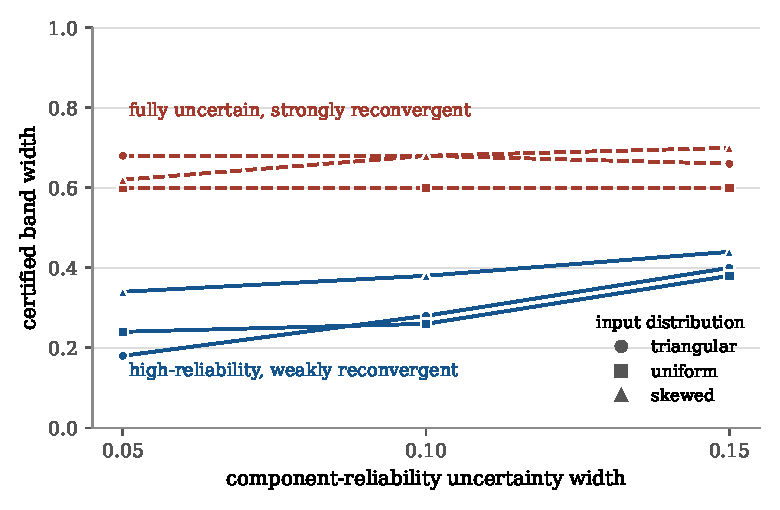
\includegraphics[width=0.8\linewidth]{envelope.pdf}
\caption{Tightness envelope of the certified p-box bound on the benchmark network: band width against
component-reliability uncertainty width, for three input-distribution shapes and two reconvergence
regimes. Soundness holds in every configuration (zero violations); only tightness varies, driven by the
regime rather than the input shape.}
\label{fig:envelope}
\end{figure}

\begin{figure}[t]\centering
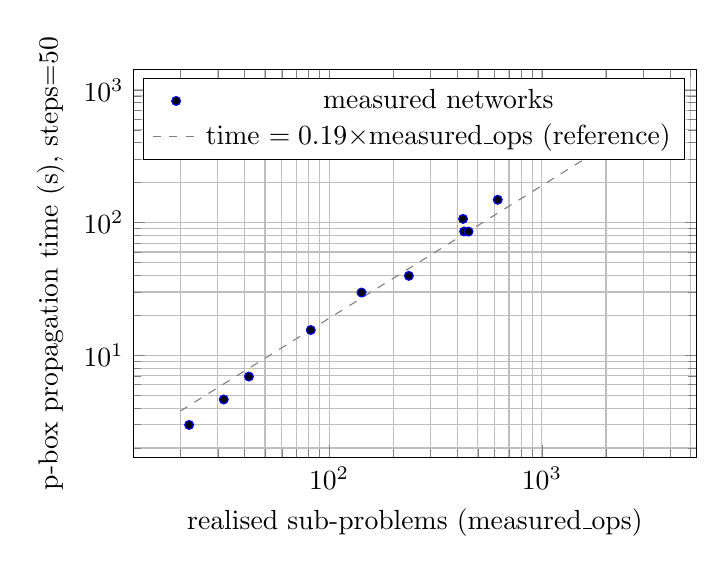
\begin{tikzpicture}
\begin{loglogaxis}[
  width=.72\linewidth, height=6.5cm,
  xlabel={realised sub-problems (measured\_ops)},
  ylabel={p-box propagation time (s), steps=50},
  grid=both,
  mark size=1.6pt,
  log basis x=10, log basis y=10,
]
\addplot+[only marks, mark=*, mark options={fill=black}] coordinates {
  (22, 2.9851)
  (32, 4.6418)
  (42, 6.9117)
  (82, 15.4937)
  (142, 29.6888)
  (237, 39.6774)
  (426, 106.6036)
  (431, 85.7466)
  (452, 85.5499)
  (620, 148.5832)
  (1564, 405.4452)
  (1747, 342.3654)
  (1961, 359.3102)
  (3112, 808.1473)
};
\addplot[domain=20:3200, samples=2, dashed, gray] {0.19*x};
\legend{measured networks, time $=0.19\times$measured\_ops (reference)}
\end{loglogaxis}
\end{tikzpicture}
\caption{p-box propagation time at a fixed discretisation level (steps=50) against the realised
sub-problem count (measured\_ops) already reported for the exact/interval cost comparison
(Section~\ref{sec:complexity}), across 14 networks spanning a 141$\times$ range in measured\_ops.
Each point is a single clean measurement (one propagation per fresh process, JIT-warmed on a
throwaway network never the target). The near-linear relationship on log-log axes
(time/measured\_ops within roughly 0.14--0.26\,s/op throughout) shows that the same realised-work
quantity governing Float64/Interval cost also governs p-box cost, at a roughly constant price per
resolved sub-problem for a given discretisation level --- not the raw conditioning-set-width bound,
which does not correlate this cleanly.}
\label{fig:pbox_cost}
\end{figure}

\subsubsection{A certified decision bound from a single propagation}\label{sec:certified}

The practical payoff is that the propagated distribution bounds certify decision-relevant probabilities.
Consider a stated reliability requirement $x^\ast$ for a given node: the propagated p-box yields
guaranteed lower and upper bounds on $P(b(v)\le x^\ast)$, the probability that the node fails its
requirement, from one propagation. On the benchmark network at a representative requirement of
$x^\ast=0.95$, the certified band on this probability had width between $0.02$ and $0.12$ across the
regimes tested (Table~\ref{tab:certified}). Matching that precision by simulation, planned conservatively
without foreknowledge of the answer, would require between $267$ and $9{,}604$ samples of the network's
uncertain inputs, and the result would remain a statistical estimate rather than a guarantee. (When the
true probability lies near $0$ or $1$ the retrospective sample requirement collapses --- correct
statistics, but knowable only in hindsight; the planning figure quoted is the one a practitioner must
budget.) An exact decision-diagram method has no analytic route to this bound at all and would itself
fall back on simulation. This certified-bound capability, not raw speed, is the concrete engineering
value of imprecise propagation.

\begin{table}[t]
\centering\small
\caption{Certified bound on the requirement-violation probability $P(b(v)\le 0.95)$ at the benchmark
network's target node, from a single propagation, against the Monte Carlo sample count required to match
the certified precision under worst-case a-priori planning.}
\label{tab:certified}
\begin{tabular}{llccc}
\toprule
Regime & Uncertainty width & Certified band & Band width & MC samples (planning)\\
\midrule
perfect components & 0.05 & [0.000, 0.020] & 0.02 & 9{,}604\\
perfect components & 0.10 & [0.000, 0.100] & 0.10 & 385\\
perfect components & 0.15 & [0.000, 0.120] & 0.12 & 267\\
uncertain components & 0.05--0.15 & [0.980, 1.000] & 0.02 & 9{,}604\\
\bottomrule
\end{tabular}
\end{table}

\subsection{Applied Case Study: A Medical Drone Logistics Network for Scotland}\label{sec:drone}

The methodology having been validated in Sections~\ref{sec:grid}--\ref{sec:imprecise}, this section
applies it to a real infrastructure planning problem: the conceptual medical drone delivery network for
Scotland designed by Jones et al.\ (2025), who optimised station placement and network structure over
real hospital, airport, and candidate-station locations, two drone types (short-range vertical take-off
and landing, nominal range 70\,km; long-range fixed-wing, nominal range 700\,km), and stated
infrastructure specifications, trading off delivery time, capital cost, and resilience. The reliability
question the present method can answer, and their point-probability framework cannot, is: given the
acknowledged uncertainty in the component availability assumptions, how confidently can each location in
a candidate design be said to be reachable from the supply hubs?

\subsubsection{Model inputs and their provenance}\label{sec:provenance}

Every input of the reliability model is derived from the source study, with one clearly flagged
extension.

\paragraph{Location availability} The source study's own resilience analysis assumes that non-hub
locations fail independently with probability $0.2$ while hub locations are always available. We adopt
the same structure, but represent the non-hub availability as the interval $[0.75,0.85]$ centred on the
source study's figure, for a deliberate reason: that figure is stated in the source study as an
assumption rather than derived from data, and an interval-valued input turns the analysis into a
built-in sensitivity assessment of precisely that assumption. Hub locations retain availability $1$.

\paragraph{Connection existence} A connection between two locations exists, for a given drone type, if
and only if the inter-location distance is within that type's stated nominal range --- the source
study's own network-construction rule, applied exactly. Where both drone types can serve a connection,
the connection is available if either type's transmission succeeds, the two being independent.

\paragraph{Connection reliability --- the flagged extension} The source study holds weather conditions
constant in its own analysis, while noting that weather-driven range variation is in principle an
uncertain quantity requiring expert elicitation, which it deliberately defers. We extend exactly this
deferred point, and only this point. A connection operating well within a drone's nominal range is
treated as reliable. A connection whose length falls within an illustrative weather-derating margin of
the range limit --- the final ten per cent, an assumed bound since the source study does not quantify
one either --- is treated as genuinely uncertain: its transmission probability is the vacuous interval
$[0,1]$, expressing honestly that adverse weather may or may not close that particular route. This is an
extension of the source study's own stated limitation, not an independent invention, and no other
probability in the model is assumed.

\paragraph{Direction of dependency} The source study's connections are undirected, since a delivery
route can be flown in either direction; the reliability question, however, concerns supply reaching
facilities from hubs. The dependency graph is therefore directed from the hub tier outward --- matching
the source study's own hub-and-spoke architecture --- and source-to-node reachability is computed on the
resulting acyclic structure.

\subsubsection{Network configurations}\label{sec:configs}

The source study's actual optimised network layouts are not published. Three configurations are
therefore constructed as proxies for the qualitative character of three trade-off points described in
its results: a fixed-wing-reliant centralised design serving remote locations through a hub backbone
(217 locations, 263 connections); a densely interconnected short-range design (242 locations, 1{,}753
connections); and a minimal-investment design retaining only pre-existing, non-optional infrastructure
(230 locations, 1{,}648 connections). Each is explicitly a proxy for the described character of the
corresponding design, not a reproduction of an unavailable optimisation result.

\subsubsection{Redundancy and the practical boundary of exact analysis}\label{sec:redundancy}

A network-design parameter controls the reconvergent structure of each configuration: the number of
alternate routes provisioned per location --- a genuine redundancy choice in network design, not a
parameter of the analysis method. Connecting every operationally plausible pair of locations makes
exact diamond identification itself impractical: identification alone exceeded the memory available on
a 16\,GB workstation and did not complete (the original submission reported computation becoming
impractical beyond a nesting depth of approximately 18, a figure the reviewers also highlighted; this
unrestricted-connectivity configuration lies beyond that figure, though its precise conditioning-set
size could not be measured, since identification itself did not finish). Bounding the provision to
sixteen alternate routes per location brought the measured requirement to 16 in both dense
configurations --- just inside the practical range identified in the original submission --- and further increases in provisioned routes
changed neither the requirement nor the runtime materially, indicating that the reconvergent structure
of this network saturates at that level. The full exact interval propagation of the densest
configurations completes in under 25 seconds; the sparse centralised configuration, whose conditioning
requirement is 10, completes in well under one second. The practical boundary of exact analysis on this
real network is thus a measured quantity, expressed in terms of a controllable design parameter: more
provisioned redundancy improves resilience but raises the cost of verifying it exactly.

The comparison of Section~\ref{sec:comparison} was repeated on these networks. On the sparse centralised
configuration the two methods agree to floating-point precision, and the one-shot interval computation
of the proposed method is approximately fourteen times faster than the decision-diagram route to the
same interval ($0.012$\,s against $0.173$\,s; diagram size 2{,}667 nodes). On the minimal-investment
topology provisioned at low redundancy (six alternate routes per location), both methods are comfortably
fast and the proposed method remains moderately faster (approximately six times: $0.128$\,s against
$0.830$\,s; diagram size 4{,}968 nodes; agreement $1.1\times10^{-16}$). On the same topology at sixteen
alternate routes per location, the decision-diagram build did not complete within a practical
computational budget under either of two variable-ordering strategies (dynamic reordering, and a fixed
topological order), while the proposed method completed the full exact computation in under 25 seconds.
We state the finding precisely: both methods are governed by the same underlying network property, and
both are practical at low redundancy; on this network, the practical range of the proposed method,
measured along a real redundancy design parameter, extends further than that of the decision-diagram
alternative. No claim is made that decision-diagram methods cannot handle this problem class in general,
nor that the crossover point has been located precisely.

\subsubsection{Reliability findings}\label{sec:findings}

Table~\ref{tab:drone} summarises the propagated interval reliabilities. They are informative, not
vacuous, and they differ meaningfully across the three designs. In the centralised, low-redundancy
configuration the propagated bounds are narrow (band width at most $0.10$, mean $0.089$): each
location's reachability essentially inherits the availability band assumed for the locations themselves,
with little additional uncertainty accumulated through the network --- but also little protection: the
design is tree-like, so single-route failures directly disconnect service. In the two higher-redundancy
configurations the best-connected locations are reachable with near-certainty, while the worst-served
locations carry a genuine, decision-relevant spread: the least certain facility --- Islay Hospital, an
island site --- has reachability probability bounded between $0.56$ and $0.72$. That interval is the
honest answer to the planning question under the acknowledged input uncertainty: no point-probability
analysis of the same design could distinguish a facility whose reachability is confidently $0.6$ from
one whose reachability is anywhere between $0.56$ and $0.72$, yet the two call for different
interventions. Figure~\ref{fig:map} maps the network coloured by the lower reliability bound and by band
width, identifying the specific facilities --- concentrated in the islands and the far north --- where
additional redundancy, or better component-availability data, would most improve either the network or
our knowledge of it.

\begin{table}[t]
\centering\small
\caption{The three proxy configurations of the applied case study: structure, conditioning requirement,
full interval-propagation soundness, and the propagated reliability bounds. Every belief is contained in
$[0,1]$ with $\underline{b}\le\overline{b}$ (soundness); the worst-served facility in both dense
configurations is Islay Hospital.}
\label{tab:drone}
\begin{tabular}{lrrrccc}
\toprule
Configuration & $|V|$ & $|E|$ & $|C|_{\max}$ & mean band & max band & worst facility\\
\midrule
fixed-wing centralised & 217 & 263 & 10 & 0.089 & 0.100 & [0.750, 0.850]\\
dense decentralised & 242 & 1753 & 16 & 0.094 & 0.161 & [0.562, 0.722]\\
concentrated minimal & 230 & 1648 & 16 & 0.093 & 0.161 & [0.562, 0.722]\\
\bottomrule
\end{tabular}
\end{table}

\begin{figure}[t]
\centering
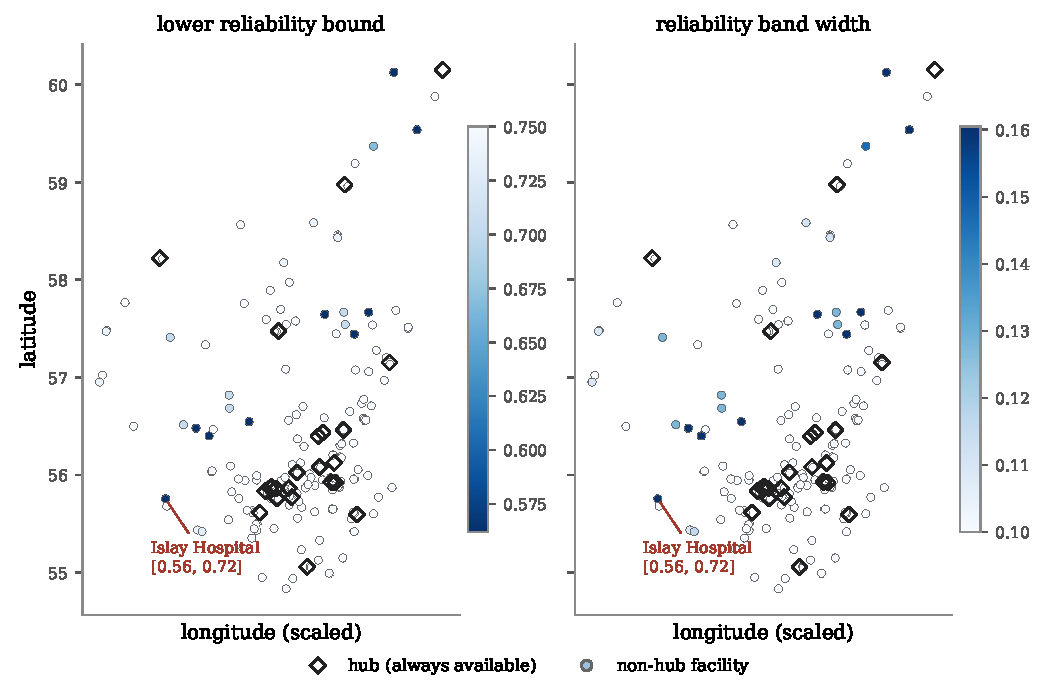
\includegraphics[width=\linewidth]{drone_reliability_map.pdf}
\caption{Reliability map of the dense decentralised configuration: each facility coloured by the lower
bound of its propagated reachability reliability (left; darker = less certainly reachable) and by the
width of its reliability band (right; darker = more uncertainty). Hubs (diamonds) are assumed always
available. Uncertainty concentrates at island and far-northern facilities; the worst-served facility,
Islay Hospital, is bounded at [0.56, 0.72].}
\label{fig:map}
\end{figure}

\subsection{Adversarial and Worst-Case Structural Complexity}\label{sec:adversarial}

The comparison of Section~\ref{sec:comparison} shows that the proposed method and a well-ordered decision
diagram are of the same order on a broad corpus of random, structured, and real networks. This section
probes the two ends of that comparison directly: a family constructed so that the method's own
factorisation (Lemma~\ref{lem:factorisation}) applies maximally, a family constructed so that it cannot
apply at all, and --- as a check that these are not merely artefacts of hand-constructed worst cases --- a
real, independently published benchmark suite subjected to the same worst-case input convention used
throughout this corpus.

\paragraph{Independent structure: the fan-in family} The family $\mathrm{fanin}\text{-}k$ consists of $k$
independent fork gadgets reconverging at a single sink. Because the gadgets share no ancestry, the
factorisation of Lemma~\ref{lem:factorisation} conditions each independently: the proposed method resolves
exactly $2k{+}1$ sub-problems for every $k$ tested ($k=2,\dots,16$), confirmed exactly on every instance,
against a diagram whose size grows as $16.0\,k^{1.49}$ under dynamic reordering. In wall-clock terms the
proposed method completes in under one millisecond throughout, against roughly one to two seconds to build
the diagram --- a three-order-of-magnitude advantage on this family, because there is no reconvergent
dependency for either method to pay for.

\paragraph{Maximal correlation: the mesh family} The family $\mathrm{mesh}\text{-}w$ is a width-$w$,
fixed-length ($L=8$) reconvergent lattice: a single genuinely correlated block with no independent
partition, the opposite extreme from fan-in. Table~\ref{tab:adversarial} reports both the realised
sub-problem count and the wall-clock time against the sifted decision diagram. The two measures tell
different stories: in sub-problem counts the diagram's advantage appears to grow to three orders of
magnitude by $w=8$, but the wall-clock gap at the same point is fifty-five-fold --- the proposed method is
faster than $w=4$ and the diagram becomes faster from $w=5$, a materially smaller and later crossover than
the raw operation count suggests, because a diagram node and a resolved sub-problem are not computationally
equivalent units of work. Between $w=8$ and $w=9$ the realised sub-problem count grows by a factor of only
$1.39$, but wall-clock time grows by a factor of $37$: the proposed method's practical boundary on this
family is set by the memory footprint of its sub-problem cache crossing available memory, not by the
growth of the sub-problem count itself, while the diagram remains untroubled at the same point (3{,}335
nodes, under four seconds). We report this as a practical-boundary observation, not a further scaling
point on the same curve.

\begin{table}[t]
\centering\small
\caption{Complexity on adversarial families: realised sub-problems (this method, with independent-diamond
factorisation) versus sifted ROBDD node count, in both operation-count and wall-clock terms.
\emph{fan-in-$k$}: independent fork gadgets; factorisation keeps both methods linear. \emph{mesh-$w$}: a
maximally correlated lattice at fixed length $L{=}8$; the diagram's advantage in raw operation count
substantially overstates its wall-clock advantage, and the $w{=}8\!\to\!9$ step is a memory-bound practical
boundary, not a further point on a smooth curve.}
\label{tab:adversarial}
\begin{tabular}{lrrrrrr}
\toprule
Family & param & ops & ROBDD nodes & time (this method) & time (ROBDD) & regime \\
\midrule
fan-in-$k$ & 8  & 17        & 474       & $<\!1$\,ms & $\sim\!1$--2\,s & method faster ($\sim\!1000\times$) \\
fan-in-$k$ & 16 & 33        & 802       & $<\!1$\,ms & $\sim\!1$--2\,s & method faster ($\sim\!1000\times$) \\
mesh-$w$   & 4  & 20{,}603     & 700       & 0.37\,s    & 1.19\,s    & method faster \\
mesh-$w$   & 5  & 170{,}001    & 805       & 3.9\,s     & 1.2\,s     & diagram faster \\
mesh-$w$   & 8  & 3{,}895{,}252 & 2{,}621   & 159.5\,s   & 2.9\,s     & diagram faster ($55\times$) \\
mesh-$w$   & 9  & 5{,}430{,}000\footnotemark & 3{,}335 & 5{,}924.7\,s & 3.8\,s & memory boundary, this method \\
\bottomrule
\end{tabular}
\end{table}
\footnotetext{Approximate: the $\times1.39$ growth factor from $w{=}8$ is reported exactly; the absolute
count is rounded.}

\paragraph{A real published benchmark under the same convention: ISCAS85} The two families above are
constructed to sit at the extremes of the method's own factorisation. To check that comparably extreme
behaviour also arises outside hand-constructed cases, we assigned the ISCAS85 combinational benchmark
circuits (Brglez and Fujiwara 1985) --- a real, widely used suite of digital logic circuits represented
natively as directed acyclic graphs --- the same illustrative, non-degenerate component reliability (0.9,
uniformly) already used for the synthetic corpus and the structured networks of Section~\ref{sec:comparison}.
This choice is itself a deliberate worst case for the method's identification procedure: the
implementation excludes a node from a conditioning set only when its reliability is fixed at exactly $0$
or $1$, since such a node's reachability state carries no residual uncertainty to enumerate; assigning
every component a non-degenerate value therefore ensures that no reconvergent structure the topology
admits is excluded from conditioning, so the full structural complexity the circuit's connectivity permits
is actually realised.
The smallest circuit, \emph{c17} (11 gates), is trivial (conditioning width 1) and was fully validated
across all three input types, including a probability-box propagation whose cost matched the prediction of
Section~\ref{sec:pbox}'s realised-work relationship closely (predicted 1.3--2.3\,s at 50 discretisation
levels; measured 1.41\,s). The next three circuits tested, \emph{c432} (196 gates), \emph{c499} (243
gates), and \emph{c880} (443 gates), reach conditioning widths of 67, 41, and 50 respectively --- an order
of magnitude beyond any other network in this corpus --- placing exact propagation on these circuits well
outside a practical budget; two further circuits, \emph{c1355} and \emph{c1908} (587 and 913 gates), exceed
the memory available on a 16\,GB workstation during identification itself. This is not evidence that the
proposed method is uniquely disadvantaged on this domain: El Fattah and Dechter (1996), studying the same
benchmark circuits with classical tree-clustering and cutset conditioning --- the general method this paper
specialises --- independently report clique and cutset sizes for \emph{c432} that they describe as "clearly
not feasible" by any exact structural method, and comparably extreme figures for the larger circuits in the
suite. Since decision-diagram size is governed by the same structural width parameter as the conditioning
width reported here (Section~\ref{sec:complexity}), a well-ordered decision diagram would be expected to
face the same difficulty on these specific circuits, not to resolve it. We report this as an honestly
located, independently corroborated boundary of exact structural inference in a fourth domain, rather than
as a limitation specific to this method.

The three findings together support a single, symmetric characterisation: every exact method pays a
structural cost somewhere, and this section identifies which resource is paid, and where, rather than
asserting that one method escapes the cost the other pays. On independent structure, the proposed method
is faster by three orders of magnitude; on maximally correlated structure, a well-ordered decision diagram
is faster by up to two; on a real published circuit family under a deliberately unfavourable input
convention, both methods --- and, independently, classical clustering and conditioning methods studied
decades earlier --- reach the same practical wall.

\subsection{Limitations and Future Work}\label{sec:limitations}

The method is exact, and we are explicit about where its advantages do and do not lie.

\paragraph{Exact point-valued reliability} The method offers no asymptotic advantage over a well-ordered
decision diagram. Both are exponential in the network's structural width --- the conditioning width
here, the pathwidth for the diagram --- reflecting the \#P-hardness of network reliability; across the
corpus neither dominates, and the realised work tracks the diagram size to within a constant factor
(Section~\ref{sec:comparison}). The method is competitive with, not superior to, a well-ordered decision
diagram for exact point evaluation; its distinctive value lies in imprecise propagation.

\paragraph{Practical range} Being exact, the method is exponential in width and intended for the
sparse-to-moderate regime --- a ceiling shared with every exact method. The applied case study makes the
boundary concrete on one real network: a conditioning requirement of 16, reached at sixteen
provisioned alternate routes per location, remains practical (tens of seconds); unrestricted connectivity,
by contrast, makes exact diamond identification itself exceed a 16\,GB memory budget before propagation
can even begin. Imprecise propagation does not relax this boundary:
interval and p-box propagation use the same conditioning depth as exact point propagation, and only a
change to the network design itself alters the cost. For networks beyond the practical range, a
depth-limited hybrid suggests itself: condition exactly to a chosen depth and, beyond it, combine
reconvergent contributions without conditioning, which for interval inputs yields a rigorous outer bound
(wider, but sound, since na\"ive interval evaluation over-approximates a monotone function) and for
p-box inputs would use the Fr\'echet combination for the unconditioned remainder. We emphasise that this
hybrid is proposed, not implemented or evaluated here; it is future work, and the method reported in
this paper does not degrade exactness anywhere.

\paragraph{Imprecise propagation} Interval results are exact at machine precision; the speed comparison
of Section~\ref{sec:interval} is scoped to one-shot queries. Distributional (p-box) bounds are sound but
their tightness is structure-dependent --- tight for high-reliability or weakly reconvergent systems,
conservative for strongly reconvergent systems with broadly uncertain components --- and their cost
grows super-linearly with the discretisation level (empirically, an exponent of approximately $2.6$,
increasing toward the higher end of the range tested --- markedly worse than quadratic), which confines
full distributional propagation to
modest networks at present; for larger networks interval propagation combined with sampling is the
practical recourse. The tighter positive-dependence conditioning operator is validated but not proven
sound; the proven Fr\'echet operator is used for every guaranteed claim, and a proof (or refutation) for
the tighter operator is an open mathematical question we have verified is not settled in the existing
dependence-bound literature.

\paragraph{Structural scope} The method addresses directed acyclic dependency structures. The applied
case study's networks are directed by the hub-and-spoke supply logic of their source design
(Section~\ref{sec:provenance}), which is the appropriate reading of that system; general cyclic or
bidirectional dependency networks --- feedback loops, return flows --- are outside the present scope,
and their principled treatment (for example by unrolling or by strongly-connected-component
condensation) is future work.

%% ============================================================================
\section{Conclusions}\label{sec:conclusions}

An exact reliability analysis method for directed acyclic process networks with reconvergent dependency
structures, the Information Propagation Algorithm (IPA), has been presented. The method computes
source-to-node reliability by propagating reachability probabilities in topological order, resolving
dependent incoming signals by conditioning on minimal separating sets of shared ancestors, and replacing
resolved fork--join substructures with statistically equivalent supernodes. The revision establishes the
method's formal position: it is a specialisation of cutset conditioning to source-to-node reachability,
its per-instance cost is exactly $\sum_d 2^{|C_d|}$ over the diamonds resolved --- computable before
enumeration --- and an independent-substructure factorisation reduces fan-in conditioning from
exponential to linear where independence permits.

Exactness was verified against an independent exact method, a reduced-ordered binary decision diagram
with dynamic variable reordering, across 129 random and mutated networks, six topological families, and
real infrastructure networks, with worst observed disagreement at floating-point precision. The same
comparison shows that the method's cost is governed by the same structural width parameter as the
diagram's size, with neither method dominating: for exact point-valued reliability the method is
competitive with, not superior to, a well-ordered decision diagram. Its distinguishing capability is the
native propagation of imprecise component reliabilities: interval-valued inputs yield the exact
reliability range at machine precision --- and, for one-shot queries, faster than the decision-diagram
route to the same interval on every family tested --- while probability-box inputs yield guaranteed
distributional bounds via a conditioning operator grounded in the Fr\'echet--Hoeffding inequalities,
enabling certified bounds on requirement-violation probabilities from a single propagation, a result no
point-valued exact method produces analytically.

An applied case study of a medical drone logistics network for Scotland, with every input traced to the
source design study and one clearly flagged extension, demonstrated the engineering use of the method:
propagated reliability bounds identify the facilities whose delivery reachability is most uncertain
under honest input uncertainty, and a sweep of a real redundancy design parameter located the practical
boundary of exact analysis on the network --- within which the method completed full exact propagation
in under 25 seconds at a redundancy level where the decision-diagram alternative did not complete within
a practical budget. Exact reliability analysis of large acyclic networks is feasible whenever
dependency-inducing substructures remain sufficiently localised, and the boundary of feasibility can be
measured and expressed in design terms rather than assumed.

Future work includes a soundness proof for the tighter positive-dependence conditioning operator, the
depth-limited hybrid scheme for networks beyond the exact range, extension to multi-state components and
explicitly modelled common-cause failures, and principled treatment of cyclic dependency structures.

\section*{Acknowledgements}
This work was supported by the Nuclear Decommissioning Authority (NDA) in conjunction with the UK National
Nuclear Laboratory (UKNNL) through the NDA Bursary Scheme (project number NNL/UA/118).

\section*{Data and Software Availability}
The implementation of the Information Propagation Algorithm (IPA) is released as the open-source Julia
package \texttt{InformationPropagationAnalysis.jl}, registered in the Julia General package registry
(current version 0.2.1) and available at
\texttt{https://github.com/Temi-Tory/InformationPropagationAnalysis.jl}. The benchmark networks,
validation scripts, and result artifacts required to reproduce every table and figure in this manuscript
are deposited at [Zenodo DOI to be inserted upon minting] under an MIT licence, together with a README
mapping each artifact to the manuscript table or figure it supports.

%% ============================================================================
\section*{References}
\begingroup
\setlength{\parindent}{-1.5em}\setlength{\leftskip}{1.5em}\small

Au, S.-K., Beck, J.L., 2001. Estimation of small failure probabilities in high dimensions by subset
simulation. Probabilistic Engineering Mechanics 16 (4), 263--277.

Billinton, R., Allan, R.N., 1992. Network modelling and evaluation of simple systems. In: Reliability
Evaluation of Engineering Systems: Concepts and Techniques. Springer US.

Brglez, F., Fujiwara, H., 1985. A neutral netlist of 10 combinational benchmark circuits and a target
translator in Fortran. In: Proceedings of the IEEE International Symposium on Circuits and Systems,
695--698.

Brace, K.S., Rudell, R.L., Bryant, R.E., 1990. Efficient implementation of a BDD package. In:
Proceedings of the 27th ACM/IEEE Design Automation Conference, 40--45.

Bryant, R.E., 1986. Graph-based algorithms for Boolean function manipulation. IEEE Transactions on
Computers C-35 (8), 677--691.

Bryant, R.E., Meinel, C., 2002. Ordered binary decision diagrams. In: Logic Synthesis and Verification.
Springer.

\v{C}epin, M., 2011. Event tree analysis. In: Assessment of Power System Reliability: Methods and
Applications. Springer London.

Distefano, S., Puliafito, A., 2007. Dynamic reliability block diagrams vs dynamic fault trees. In: 2007
Proceedings --- Annual Reliability and Maintainability Symposium, 71--76.

Ebeling, C.E., 2019. An Introduction to Reliability and Maintainability Engineering, third ed. Waveland
Press.

El Fattah, Y., Dechter, R., 1996. An evaluation of structural parameters for probabilistic reasoning:
results on benchmark circuits. In: Proceedings of the Conference on Uncertainty in Artificial
Intelligence (UAI-96), 244--251.

Ferson, S., Kreinovich, V., Ginzburg, L., Myers, D.S., Sentz, K., 2003. Constructing Probability Boxes
and Dempster--Shafer Structures. Sandia National Laboratories, SAND2002-4015.

Fishman, G.S., 1986. A comparison of four Monte Carlo methods for estimating the probability of s--t
connectedness. IEEE Transactions on Reliability 35 (2), 145--155.

George-Williams, H., Santhosh, T.V., Patelli, E., 2021. Simulation Methods for the Analysis of Complex
Systems. Springer.

Hui, K.-P., 2007. Monte Carlo network reliability ranking estimation. IEEE Transactions on Reliability
56 (1), 50--57.

Jones, D., Filippi, G., Basu, S., Parsonage, B., Patelli, E., Maddock, C., Vasile, M., Fossati, M.,
2025. Conceptual design of a medical drone logistics network for Scotland. International Journal of
Logistics Research and Applications (submitted). \emph{[Author note: update publication status at
proof stage.]}

Kim, Y., Kang, W.-H., 2013. Network reliability analysis of complex systems using a
non-simulation-based method. Reliability Engineering \& System Safety 110, 80--88.

Kumar, T.B., Sekhar, O.C., Ramamoorty, M., 2018. Composite power system reliability evaluation using
modified minimal cut set approach. Alexandria Engineering Journal 57 (4), 2521--2528.

Lauritzen, S.L., Spiegelhalter, D.J., 1988. Local computations with probabilities on graphical
structures and their application to expert systems. Journal of the Royal Statistical Society, Series B
50 (2), 157--224.

Li, H., Zhao, Q., 2005. A cut/tie set method for reliability evaluation of control systems. In:
Proceedings of the 2005 American Control Conference, 1048--1053.

Liu, W., Li, J., 2012. An improved cut-based recursive decomposition algorithm for reliability analysis
of networks. Earthquake Engineering and Engineering Vibration 11 (1), 1--10.

Mosleh, A., 1993. Estimation of parameters of common cause failure models. In: Reliability and Safety
Assessment of Dynamic Process Systems. Springer.

Murphy, K., Weiss, Y., Jordan, M., 2013. Loopy belief propagation for approximate inference: an
empirical study. In: Proceedings of the 15th Conference on Uncertainty in Artificial Intelligence.

Pearl, J., 1988. Probabilistic Reasoning in Intelligent Systems: Networks of Plausible Inference.
Morgan Kaufmann.

Rausand, M., 2014. Reliability quantification. In: Reliability of Safety-Critical Systems. John Wiley
\& Sons.

Rauzy, A., 1993. New algorithms for fault trees analysis. Reliability Engineering \& System Safety 40
(3), 203--211.

Sherwin, D.J., Bossche, A., 1993. Fault trees, event trees and success trees. In: The Reliability,
Availability and Productiveness of Systems. Springer Netherlands.

Tong, Y., Tien, I., 2019. Probability propagation method for reliability assessment of acyclic directed
networks. ASCE-ASME Journal of Risk and Uncertainty in Engineering Systems, Part A: Civil Engineering 5
(3), 04019011.

Williamson, R.C., Downs, T., 1990. Probabilistic arithmetic I: numerical methods for calculating
convolutions and dependency bounds. International Journal of Approximate Reasoning 4 (2), 89--158.

Xing, L., Amari, S.V., 2008. Fault tree analysis. In: Handbook of Performability Engineering. Springer
London.

Yedidia, J.S., Freeman, W.T., Weiss, Y., 2003. Understanding belief propagation and its
generalizations. In: Exploring Artificial Intelligence in the New Millennium. Morgan Kaufmann.

\endgroup

\end{document}
